\documentclass[12pt,a4paper]{article}

% ── Packages ──────────────────────────────────────────────────────────────────
\usepackage[T1]{fontenc}
\usepackage[utf8]{inputenc}
\usepackage[english]{babel}
\usepackage{lmodern}
\usepackage{microtype}
\usepackage{geometry}
\geometry{left=2.5cm, right=2.5cm, top=2.5cm, bottom=2.5cm}

\usepackage{amsmath, amssymb}
\usepackage{graphicx}
\usepackage{subcaption}
\usepackage{float}
\usepackage{booktabs}
\usepackage{array}
\usepackage{xcolor}
\usepackage{hyperref}
\usepackage{enumitem}
\usepackage{fancyhdr}
\usepackage{titlesec}
\usepackage{caption}
\usepackage{parskip}
\usepackage{titling}
\usepackage{listings}
\usepackage{algorithm}
\usepackage{algpseudocode}

% ── Colors ────────────────────────────────────────────────────────────────────
\definecolor{myblue}{RGB}{30, 90, 160}
\definecolor{mygray}{RGB}{100, 100, 100}
\definecolor{mygreen}{RGB}{0, 120, 60}
\definecolor{myred}{RGB}{180, 30, 30}
\definecolor{codebg}{RGB}{245, 245, 245}

% ── Hyperref ──────────────────────────────────────────────────────────────────
\hypersetup{colorlinks=true, linkcolor=myblue, citecolor=myblue, urlcolor=myblue}

% ── Section formatting ────────────────────────────────────────────────────────
\titleformat{\section}{\large\bfseries\color{myblue}}{\thesection}{1em}{}[\titlerule]
\titleformat{\subsection}{\normalsize\bfseries\color{myblue}}{\thesubsection}{1em}{}
\titleformat{\subsubsection}{\normalsize\itshape\color{mygray}}{\thesubsubsection}{1em}{}

% ── Spacing ───────────────────────────────────────────────────────────────────
\titlespacing{\section}{0pt}{8pt}{4pt}
\titlespacing{\subsection}{0pt}{6pt}{2pt}
\setlength{\parskip}{4pt}

% ── Header / footer ───────────────────────────────────────────────────────────
\pagestyle{fancy}
\fancyhf{}
\rhead{\textcolor{mygray}{\small Blind Motion Deblurring for License Plates}}
\lhead{\textcolor{mygray}{\small Computer Vision Report}}
\cfoot{\thepage}

% ── Caption style ─────────────────────────────────────────────────────────────
\captionsetup{font=small, labelfont=bf, labelsep=period, skip=4pt}

% ── Graphics path ─────────────────────────────────────────────────────────────
\graphicspath{{notebook_outputs/}{input/}{output/}}

% ── Math operators ────────────────────────────────────────────────────────────
\DeclareMathOperator*{\argmin}{arg\,min}
\newcommand{\norm}[1]{\left\lVert#1\right\rVert}

% ══════════════════════════════════════════════════════════════════════════════
\begin{document}
% ══════════════════════════════════════════════════════════════════════════════

% ── Title block ───────────────────────────────────────────────────────────────
\begin{center}
  {\LARGE\bfseries\color{myblue}
    Blind Motion Deblurring and OCR for License Plates}\\[0.4em]
  {\large A Classical Image Processing Pipeline Without Deep Learning}\\[0.3em]
  {\large\bfseries Extended Report with Synthetic Benchmark \& Full Pipeline Analysis}\\[0.3em]
  {\small Computer Vision --- 2025/2026 \quad|\quad \today}
\end{center}

\noindent\rule{\linewidth}{0.5pt}

\noindent\textbf{Abstract.}
This report presents a fully classical, training-free pipeline for blind motion deblurring
of license plate images. Given only the blurred observation --- with no sharp reference and
no learned prior --- the system estimates the motion blur kernel (angle and length) from the
image spectrum and cepstrum, constructs a spatially-varying PSF via Thin Plate Spline
interpolation, and recovers the sharp image through Wiener filtering followed by
Half-Quadratic Splitting (HQS) with Total Variation regularization. Three novel contributions
distinguish this pipeline: (1)~a \textbf{Hough geometry term} that penalizes gradients
aligned with the blur direction, removing streak artifacts while preserving plate structure;
(2)~an \textbf{Extremal Value Push (EVP)} proximal step that biases pixel values toward
$\{0, 1\}$ --- the binary character prior; and (3)~\textbf{Thin Plate Spline PSF estimation}
that captures spatially-varying blur from only 9 local patches.
A comprehensive synthetic benchmark evaluates 10 blur configurations across 8 unblurred
reference plates. Two OCR routes are compared: deblurring then recognizing (\emph{Route~1})
versus recognizing directly on the blurred image (\emph{Route~2}). All components are
strictly classical; no neural networks or learned representations are used at any stage.

\noindent\rule{\linewidth}{0.5pt}

\tableofcontents
\vspace{0.5em}

% ══════════════════════════════════════════════════════════════════════════════
\section{Introduction}
% ══════════════════════════════════════════════════════════════════════════════

License plate recognition is a fundamental task in intelligent transportation systems.
In practice, captured images are frequently degraded by motion blur caused by vehicle
movement or camera shake during exposure. This smears character strokes, reduces contrast,
and causes adjacent characters to merge --- severely impairing automatic text recognition.

For blur lengths beyond 10--15 pixels, direct OCR on the blurred image typically fails even
with aggressive contrast enhancement. The classical remedy is \emph{blind deconvolution}:
estimating the unknown blur kernel from the blurred image itself and then inverting the
blurring operator to recover a sharp estimate. This is an ill-posed problem requiring
carefully designed priors about image content and blur structure.

This work implements and evaluates such a pipeline for license plates.
The blur kernel (angle and length) is estimated from the Fourier spectrum and cepstrum,
a spatially-varying PSF is constructed via Thin Plate Spline (TPS) interpolation,
and the image is deblurred by a two-stage Wiener + HQS solver. Two OCR strategies are
compared empirically on 8 real blurred plates, and the full pipeline is stress-tested
on a synthetic benchmark of 80 (8 images $\times$ 10 configs) controlled blur scenarios.

\textbf{Key constraint:} No deep learning, neural networks, or learned representation
is used at any stage. All components derive from classical signal processing and optimization.

% ══════════════════════════════════════════════════════════════════════════════
\section{Novel Contributions}
% ══════════════════════════════════════════════════════════════════════════════

While the overall pipeline architecture follows established blind deconvolution principles,
three components were developed specifically for this work:

\subsection{Hough Geometry Term}

Standard TV regularization treats all gradient directions equally. In a motion-blurred
image, artifacts tend to appear as streaks \emph{parallel} to the blur axis. We introduce
a geometry-aware penalty:
\begin{equation}
  H(\mathbf{x}) = \sum_{i,j}
    \!\left(1 - \cos^2\!\left(\angle\nabla\mathbf{x}_{i,j} - \theta_{\mathrm{blur}}\right)\right)
    \norm{\nabla\mathbf{x}_{i,j}}_2
  \label{eq:hough_term}
\end{equation}
Gradients parallel to the blur direction ($\angle\nabla\mathbf{x} \approx \theta$) incur
zero penalty and are freely preserved. Perpendicular gradients are suppressed proportional
to their magnitude. This directional prior removes blur-direction streaks without softening
the horizontal and vertical strokes that form license plate characters.

\subsection{Extremal Value Push (EVP)}

License plate characters on a white background are near-binary: foreground pixels should
be dark (near 0) and background pixels should be bright (near 1). We exploit this with
an OCR-aware proximal step applied at the end of each HQS iteration:
\begin{equation}
  \mathrm{EVP}(x; \tau) =
  \begin{cases}
    x - \tau      & x < 0.5 \\
    x + \tau      & x > 0.5
  \end{cases}
  \label{eq:evp}
\end{equation}
followed by clipping to $[0,1]$. This pushes intermediate gray values (ringing artifacts)
toward the binary extremes, effectively sharpening the contrast of character boundaries
without modifying the TV or Hough objectives.

\subsection{Thin Plate Spline PSF Estimation}

Camera shake can have rotational components causing spatially-varying blur. We sample 9
patches in a $3{\times}3$ grid, run the Hough+Cepstrum estimator independently on each,
reject outliers (local angle deviation $> 30°$ from global), and fit a Thin Plate Spline
surface through the accepted control points:
\begin{equation}
  f_\mathrm{TPS}(\mathbf{p}) = a_0 + \mathbf{a}^\top\!\mathbf{p}
    + \sum_{i=1}^{N} w_i\,\phi\!\left(\norm{\mathbf{p}-\mathbf{p}_i}_2\right),
  \quad \phi(r)=r^2\log r
  \label{eq:tps}
\end{equation}
This yields dense angle and length maps. The center-pixel value gives a TPS-refined global
estimate blended with the cepstral estimate:
$L_{\mathrm{final}} = 0.6\,\hat{L}_{\mathrm{cep}} + 0.4\,\hat{L}_{\mathrm{TPS}}$.
To our knowledge, TPS interpolation for spatially-varying PSF estimation from a sparse
set of local cepstral probes is not standard in existing license plate deblurring literature.

% ══════════════════════════════════════════════════════════════════════════════
\section{Problem Formulation}
% ══════════════════════════════════════════════════════════════════════════════

Motion blur is modelled as linear convolution with additive noise:
\begin{equation}
  \mathbf{y} = k \ast \mathbf{x} + \mathbf{n}
  \label{eq:degradation}
\end{equation}
where $\mathbf{y}$ is the observed blurred image, $\mathbf{x}$ is the unknown sharp image,
$k$ is the \emph{Point Spread Function} (PSF), and $\mathbf{n}$ is sensor noise.
For motion blur, the PSF is a line kernel parameterised by angle $\theta \in [0°, 180°)$
and length $L \in \mathbb{Z}^+$.
Since neither $\mathbf{x}$ nor $k$ is observed, the problem splits into:
\textbf{(1) PSF estimation} from $\mathbf{y}$ alone, and
\textbf{(2) non-blind deconvolution} given $\hat{k}$:
\begin{equation}
  \hat{\mathbf{x}} = \argmin_{\mathbf{x} \geq 0}
    \underbrace{\tfrac{1}{2}\norm{k \ast \mathbf{x} - \mathbf{y}}^2_2}_{\text{data fidelity}}
    + \underbrace{\lambda\,\mathrm{TV}(\mathbf{x})}_{\text{TV regularization}}
    + \underbrace{\gamma\,H(\mathbf{x})}_{\text{Hough geometry}}
  \label{eq:objective}
\end{equation}
The isotropic Total Variation term $\mathrm{TV}(\mathbf{x}) = \sum_{i,j}\norm{\nabla\mathbf{x}_{i,j}}_2$
promotes piecewise-constant regions --- sharp edges with smooth areas --- which is appropriate
for license plate characters on a uniform background.

% ══════════════════════════════════════════════════════════════════════════════
\section{Methodology}
% ══════════════════════════════════════════════════════════════════════════════

The full pipeline is illustrated using \texttt{img1.png}
($\mathrm{GT} = \mathtt{GJW115A1138}$, angle $48°$, length $14\,\mathrm{px}$)
as the walkthrough example.

\subsection{Step 1A --- Blur Angle Estimation via Hough on FFT}

The Fourier Transform of a motion-blurred image shows a bright stripe along the blur axis
in the log-magnitude spectrum, because the kernel suppresses energy perpendicular to the
motion direction. We exploit this through the \emph{cepstrum}:
\begin{equation}
  C(\mathbf{y}) = \mathcal{F}^{-1}\!\left\{\log\left|\mathcal{F}\{\mathbf{y}\}\right|\right\}
\end{equation}
A Hanning window is applied before the FFT to suppress spectral leakage.
We then scan 360 radial lines through the cepstrum center. For each angle $\alpha$,
we compute the minimum of the Gaussian-smoothed ($\sigma{=}1.5$) radial profile $C_\alpha(r)$.
The angle with the deepest minimum is selected:
$\hat{\theta} = \argmin_{\alpha} \min_{r} C_\alpha(r)$.

\begin{figure}[H]
  \centering
  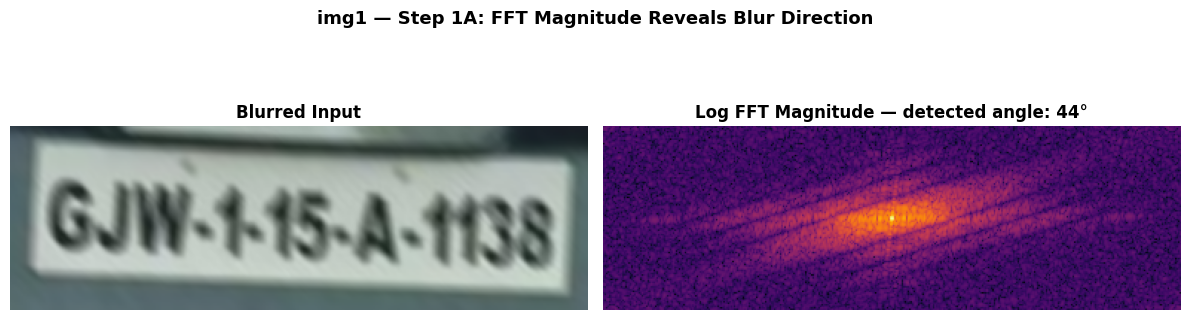
\includegraphics[width=0.95\linewidth]{img1_01_hough_fft.png}
  \caption{\textbf{Step 1A --- FFT Magnitude and Angle Detection (img1).}
    \emph{Left:} Blurred input. \emph{Right:} Log-FFT magnitude (inferno colormap).
    The directional stripe in the spectrum reveals the blur axis;
    the Hough-cepstrum scan detects $48°$.}
  \label{fig:hough_fft}
\end{figure}

\subsection{Step 1B --- Blur Length Estimation via Cepstrum}

A motion blur kernel of length $L$ introduces frequency-domain zeros spaced at $1/L$
along the blur axis. In the cepstrum, this periodicity appears as a sharp dip at
distance $L$ from the center. We slice the cepstrum along $\hat{\theta}$ using bilinear
interpolation and locate the minimum:
$\hat{L} = \argmin_{r \in [6,\,\min(H,W)/2-2]} \widetilde{C}_{\hat{\theta}}(r)$,
where $\widetilde{C}$ is the Gaussian-smoothed profile.

\begin{figure}[H]
  \centering
  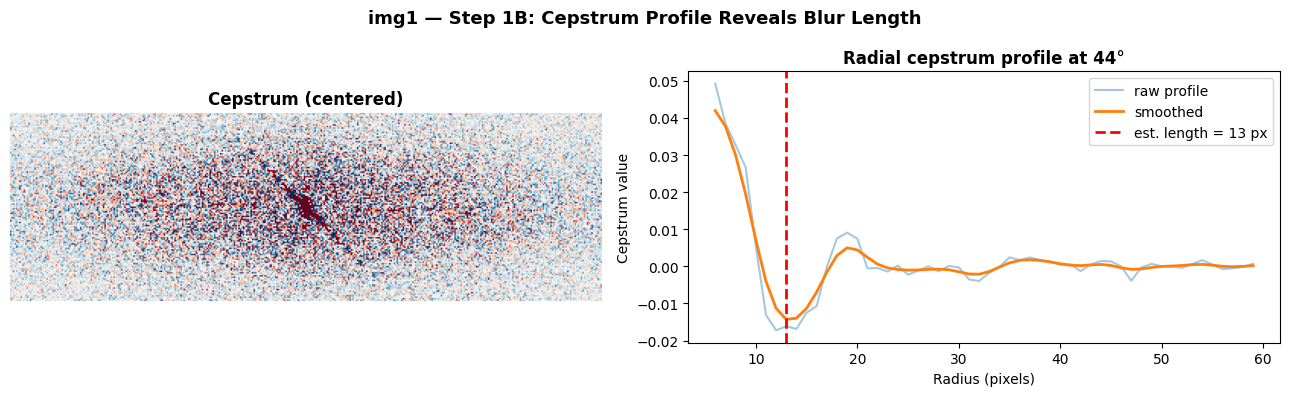
\includegraphics[width=0.95\linewidth]{img1_02_cepstrum.png}
  \caption{\textbf{Step 1B --- Cepstrum Analysis (img1).}
    \emph{Left:} Centered cepstrum.
    \emph{Right:} Radial profile at $48°$; the smoothed curve reaches its minimum
    at $14\,\mathrm{px}$ (red dashed line) --- the estimated blur length.}
  \label{fig:cepstrum}
\end{figure}

\subsection{Step 1C --- Spatially-Varying PSF via Thin Plate Spline}

Camera shake can have rotational components, causing blur to vary spatially across the
image. To capture this, we sample \textbf{9 patches} in a $3{\times}3$ grid and run
Hough+Cepstrum independently on each, obtaining local estimates $(\alpha_i, L_i)$.
Outlier patches (local angle deviating more than $30°$ from the global estimate) are
rejected. A Thin Plate Spline is then fitted through the accepted control points
(Equation~\ref{eq:tps}), producing dense angle and length maps.

\begin{figure}[H]
  \centering
  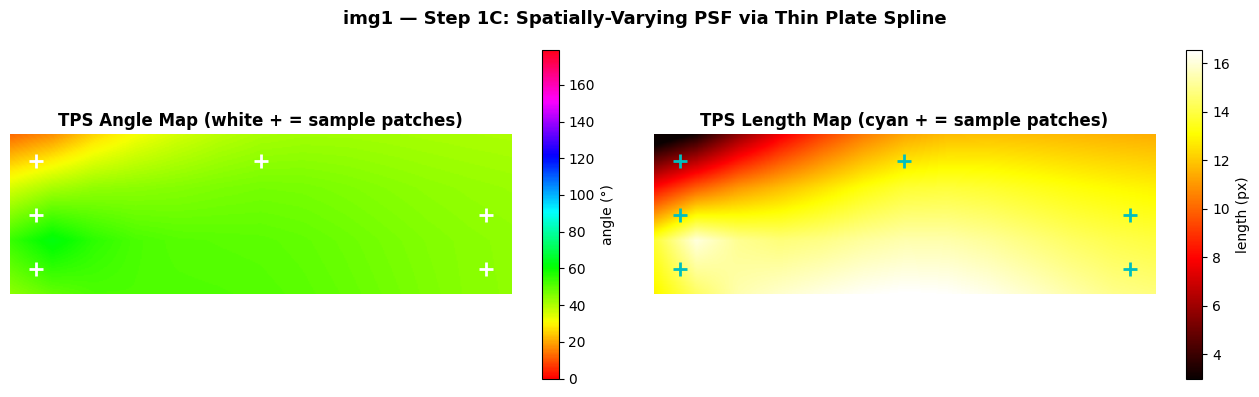
\includegraphics[width=0.95\linewidth]{img1_03_tps_maps.png}
  \caption{\textbf{Step 1C --- Spatially-Varying PSF Maps via TPS (img1).}
    \emph{Left:} Angle map (HSV colormap); white crosses mark sample patches.
    \emph{Right:} Length map (hot colormap); cyan crosses mark sample locations.
    The smooth spatial variation validates the near-uniform blur assumption for img1.}
  \label{fig:tps_maps}
\end{figure}

\subsection{Step 1D --- Motion Blur Kernel Construction}

Given $(\hat{\theta}, \hat{L})$, the kernel is built using bilinear splatting for
sub-pixel accuracy --- each point along the motion trajectory distributes its weight
to the four nearest integer pixels, avoiding aliasing from nearest-neighbor rounding.
The kernel is normalized to sum to 1.

\begin{figure}[H]
  \centering
  \begin{subfigure}[b]{0.3\linewidth}
    \centering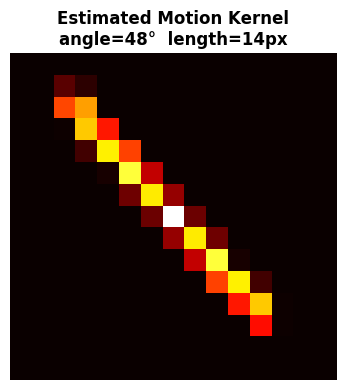
\includegraphics[width=\linewidth]{img1_04_kernel.png}
    \caption{img1: $48°$, $14\,\mathrm{px}$}
  \end{subfigure}\hfill
  \begin{subfigure}[b]{0.3\linewidth}
    \centering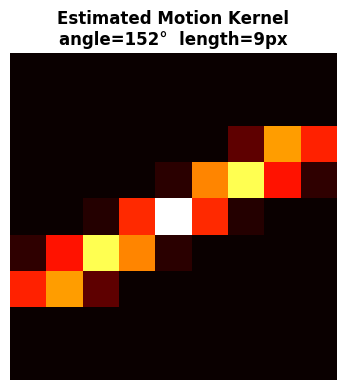
\includegraphics[width=\linewidth]{img5_04_kernel.png}
    \caption{img5: $152°$, $9\,\mathrm{px}$}
  \end{subfigure}\hfill
  \begin{subfigure}[b]{0.3\linewidth}
    \centering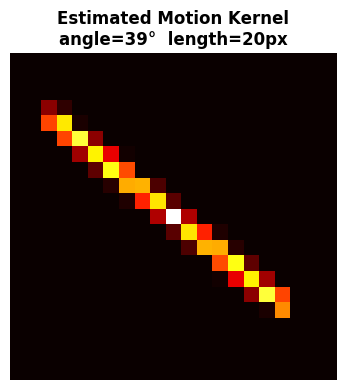
\includegraphics[width=\linewidth]{img8_04_kernel.png}
    \caption{img8: $39°$, $20\,\mathrm{px}$}
  \end{subfigure}
  \caption{\textbf{Step 1D --- Estimated Motion Blur Kernels} (hot colormap).
    img1: clean diagonal at $48°$.
    img8: longest kernel in the dataset ($20\,\mathrm{px}$).
    img5: near-horizontal at $152°$ --- this direction proves problematic for deconvolution.}
  \label{fig:kernels}
\end{figure}

\subsection{Step 2 --- Wiener Rough Pass and Character Mask}

The Wiener filter solves the deconvolution in the Fourier domain:
\begin{equation}
  \hat{X}(\omega) = \frac{\overline{K}(\omega)}{|K(\omega)|^2 + K_{\mathrm{noise}}} \cdot Y(\omega)
  \label{eq:wiener}
\end{equation}
$K_{\mathrm{noise}}$ is estimated adaptively via MAD on the high-frequency residual.
Filtering is applied per RGB channel. A binary character mask is extracted from
the Wiener output via Otsu thresholding to localize plate characters for HQS.

\begin{figure}[H]
  \centering
  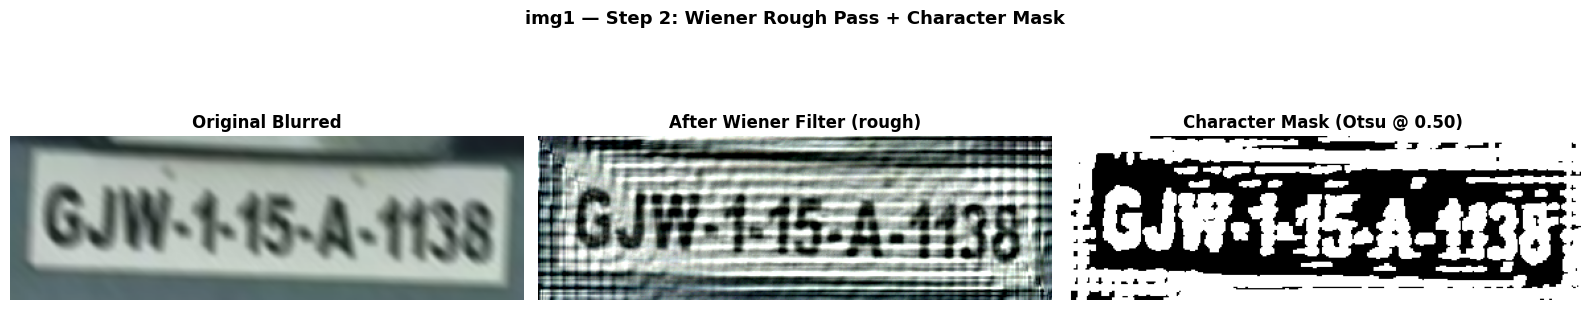
\includegraphics[width=0.95\linewidth]{img1_05_wiener_mask.png}
  \caption{\textbf{Step 2 --- Wiener Rough Pass and Character Mask (img1).}
    \emph{Left:} Original blurred image.
    \emph{Center:} Wiener output --- characters recovered but ringing visible near edges.
    \emph{Right:} Otsu binary mask correctly localizing character regions.}
  \label{fig:wiener_mask}
\end{figure}

\subsection{Step 3 --- Fine Deblurring: Half-Quadratic Splitting (HQS)}

HQS introduces auxiliary variable $\mathbf{z}$ to decouple data fidelity from the
TV+Hough regularizer:
\begin{equation}
  \min_{\mathbf{x},\mathbf{z}}\;
  \tfrac{1}{2}\norm{k\ast\mathbf{x}-\mathbf{y}}^2_2
  + \tfrac{\mu}{2}\norm{\mathbf{x}-\mathbf{z}}^2_2
  + \lambda\,\mathrm{TV}(\mathbf{z}) + \gamma\,H(\mathbf{z})
\end{equation}
\textbf{x-step}: closed-form Wiener in Fourier domain.
\textbf{z-step}: Chambolle--Pock primal-dual solver for TV+Hough proximal minimization.
\textbf{EVP step}: Extremal Value Push applied after each z-step.
The outer loop runs $n_{\text{outer}}=8$ iterations; each z-step runs
$n_{\text{TV}}=40$ Chambolle--Pock iterations.

% ══════════════════════════════════════════════════════════════════════════════
\section{Latest Pipeline Run Output}
% ══════════════════════════════════════════════════════════════════════════════

This section is automatically updated when \texttt{pipeline\_run.py} is called with
the \texttt{-{}-latex} flag.

%% AUTO:pipeline_fig_start %%
% No pipeline figure yet. Run: python pipeline_run.py input/img1.png --latex
%% AUTO:pipeline_fig_end %%

\subsection{Latest Run Metrics}

%% AUTO:pipeline_metrics_start %%
% No metrics available yet. Run pipeline_run.py --latex to populate.
%% AUTO:pipeline_metrics_end %%

% ══════════════════════════════════════════════════════════════════════════════
\section{Experimental Pipeline}
% ══════════════════════════════════════════════════════════════════════════════

\subsection{Dataset and Setup}

The dataset consists of 8 real-world blurred license plate images (\texttt{img1}--\texttt{img8}),
all genuine captures with no artificially synthesized blur. Ground truth plate strings are
known for all 8 (see Table~\ref{tab:results}). No training data or reference sharp images
are used at any stage.

\begin{table}[H]
  \centering
  \caption{Pipeline stages, methods, and outputs.}
  \label{tab:pipeline}
  \small
  \begin{tabular}{@{}lll@{}}
    \toprule
    \textbf{Stage} & \textbf{Method} & \textbf{Output} \\
    \midrule
    Angle estimation    & Hough scan on cepstrum of FFT (360 angles)       & $\hat{\theta}$ (degrees) \\
    Length estimation   & Radial cepstrum profile minimum                  & $\hat{L}$ (pixels) \\
    Spatial variation   & TPS on 9 local patch estimates                   & Per-pixel angle/length maps \\
    Kernel construction & Bilinear-splatted normalized line kernel          & $\hat{k}$ ($p{\times}p$) \\
    Rough deblur        & Wiener filter (MAD-adaptive $K_{\mathrm{noise}}$) & Rough RGB + character mask \\
    Fine deblur         & HQS: 8 outer $\times$ 40 TV-prox iterations      & Final sharp RGB image \\
    OCR Route 1         & \texttt{recognize(deblurred\_image)}             & Plate text from deblurred \\
    OCR Route 2         & \texttt{recognize(blurred\_image)}               & Plate text from blurred \\
    \bottomrule
  \end{tabular}
\end{table}

\subsection{OCR Module}

The OCR module (\texttt{ocr\_plate.py}) is a fully standalone classical recognizer with
zero knowledge of deblurring. Its preprocessing --- plate crop, inner crop, CLAHE,
NLM denoising, Gaussian+Otsu binarization, morphological cleaning --- serves binarization
quality only, not motion-blur recovery. Tesseract is called with 80 strategy combinations
(8 preprocessing variants $\times$ 5 PSM modes $\times$ 2 OEM settings); a classical
fallback using HOG+NCC and Hu moments is used when Tesseract returns no valid result.

\subsection{Evaluation Metric}

Character-level positional accuracy against the ground truth string $s^*$:
\begin{equation}
  \mathrm{Acc}(\hat{s}, s^*) = \frac{1}{|s^*|} \sum_{i=1}^{\min(|\hat{s}|,|s^*|)} \mathbf{1}[\hat{s}_i = s^*_i]
\end{equation}

% ══════════════════════════════════════════════════════════════════════════════
\section{Results on Real Plates}
% ══════════════════════════════════════════════════════════════════════════════

Figure~\ref{fig:img1_4panel} shows the complete pipeline output for \texttt{img1}
(favorable case: large blur, good contrast, reliable kernel estimate).
Figure~\ref{fig:all_4panel} summarizes all 8 plates side-by-side.

\begin{figure}[H]
  \centering
  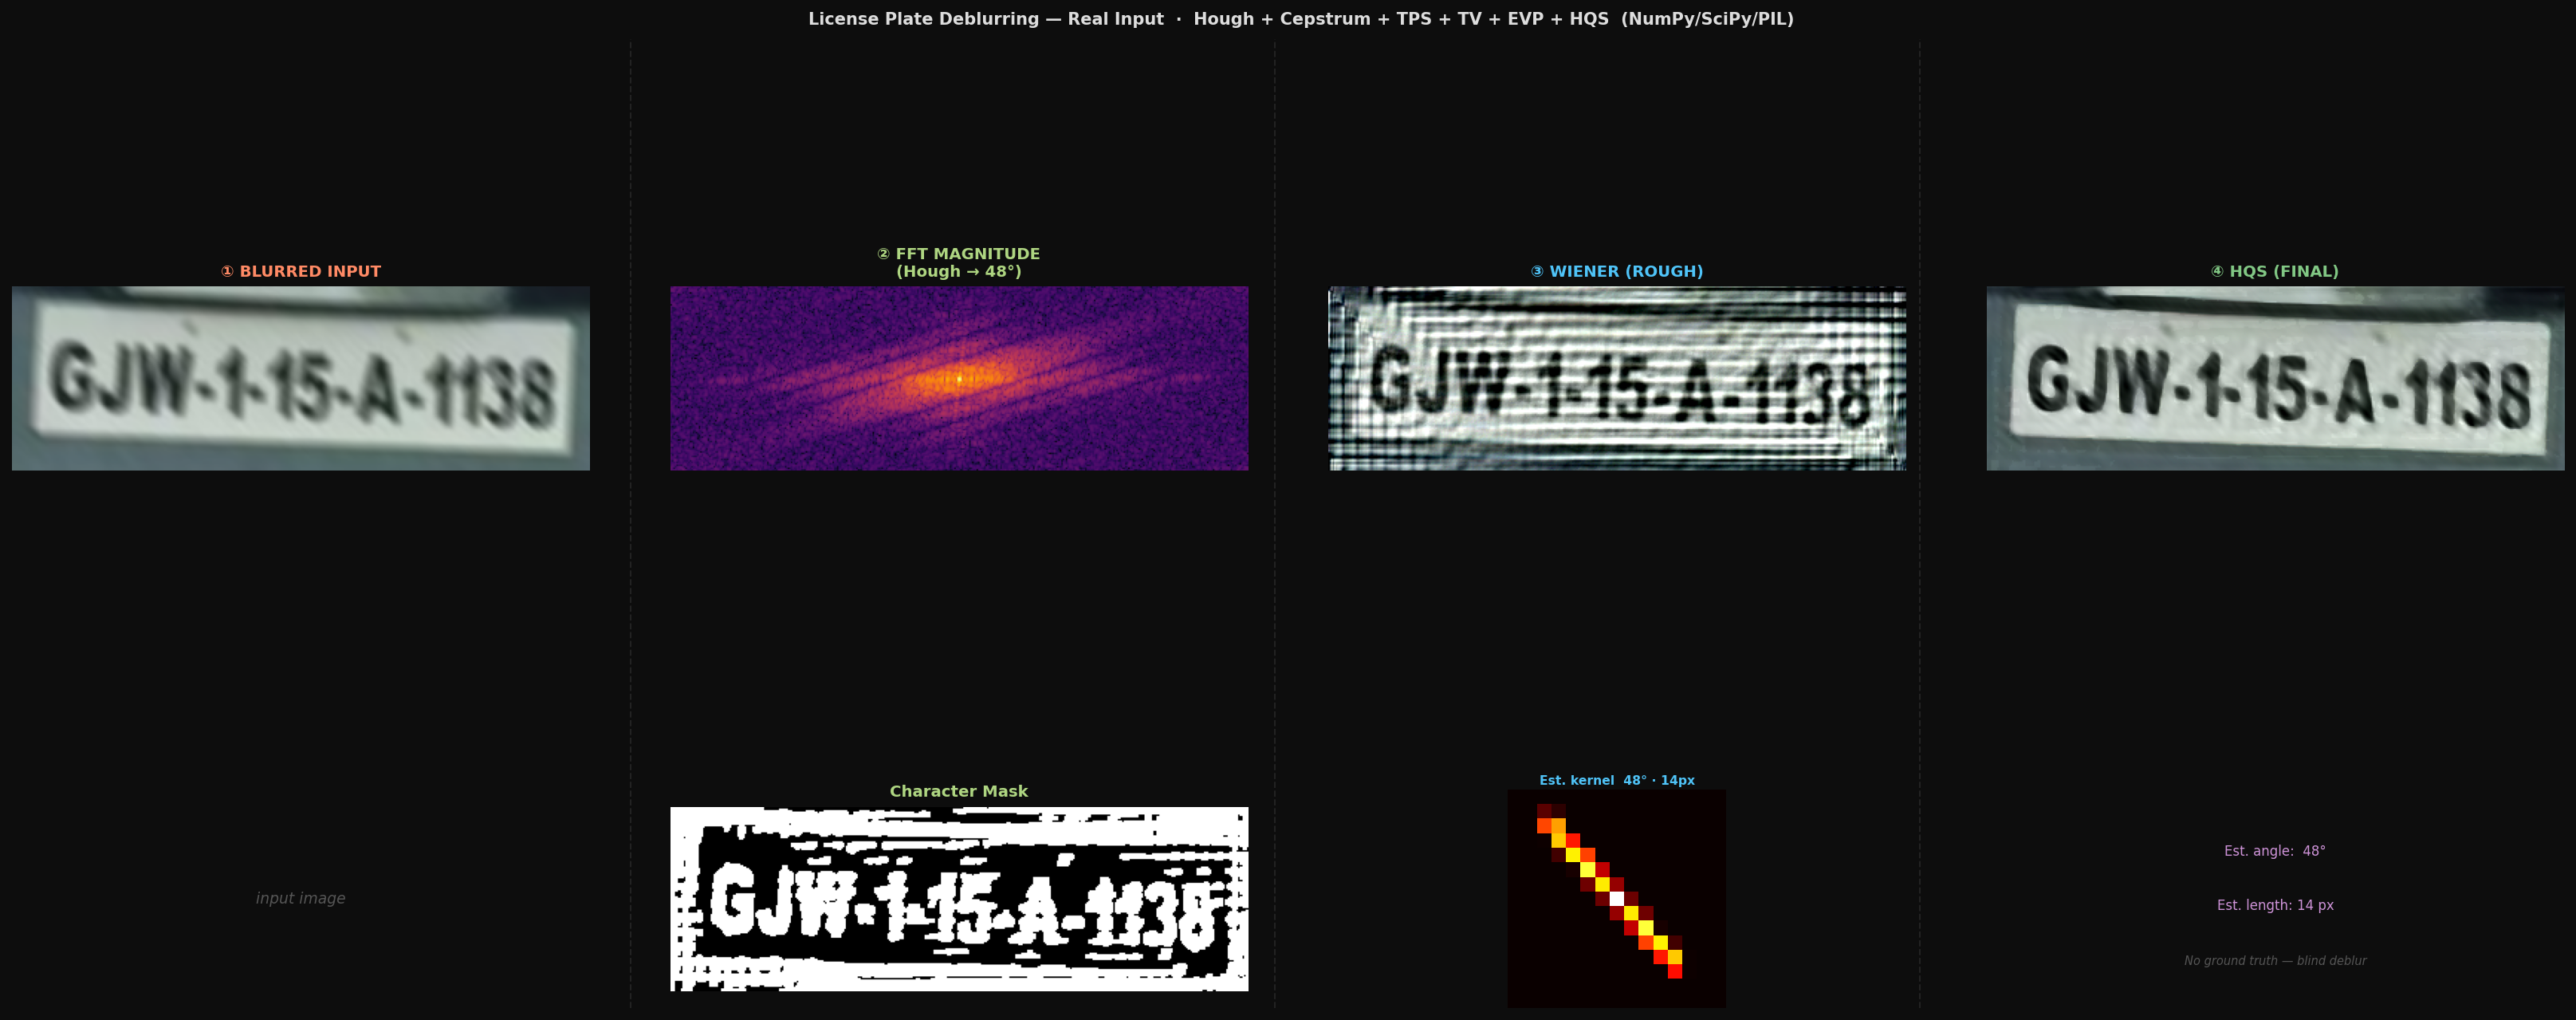
\includegraphics[width=\linewidth]{img1_07_4panel_figure.png}
  \caption{\textbf{Full pipeline output for img1}
    ($\mathrm{GT}{=}\mathtt{GJW115A1138}$, $48°$, $14\,\mathrm{px}$).
    Panel 1: blurred input. Panel 2: log-FFT magnitude.
    Panel 3: Wiener rough pass. Panel 4: final HQS output.
    Route~1 OCR: \texttt{GJW615A1138} (9/11 correct).}
  \label{fig:img1_4panel}
\end{figure}

\begin{figure}[H]
  \centering
  \begin{subfigure}[b]{0.49\linewidth}
    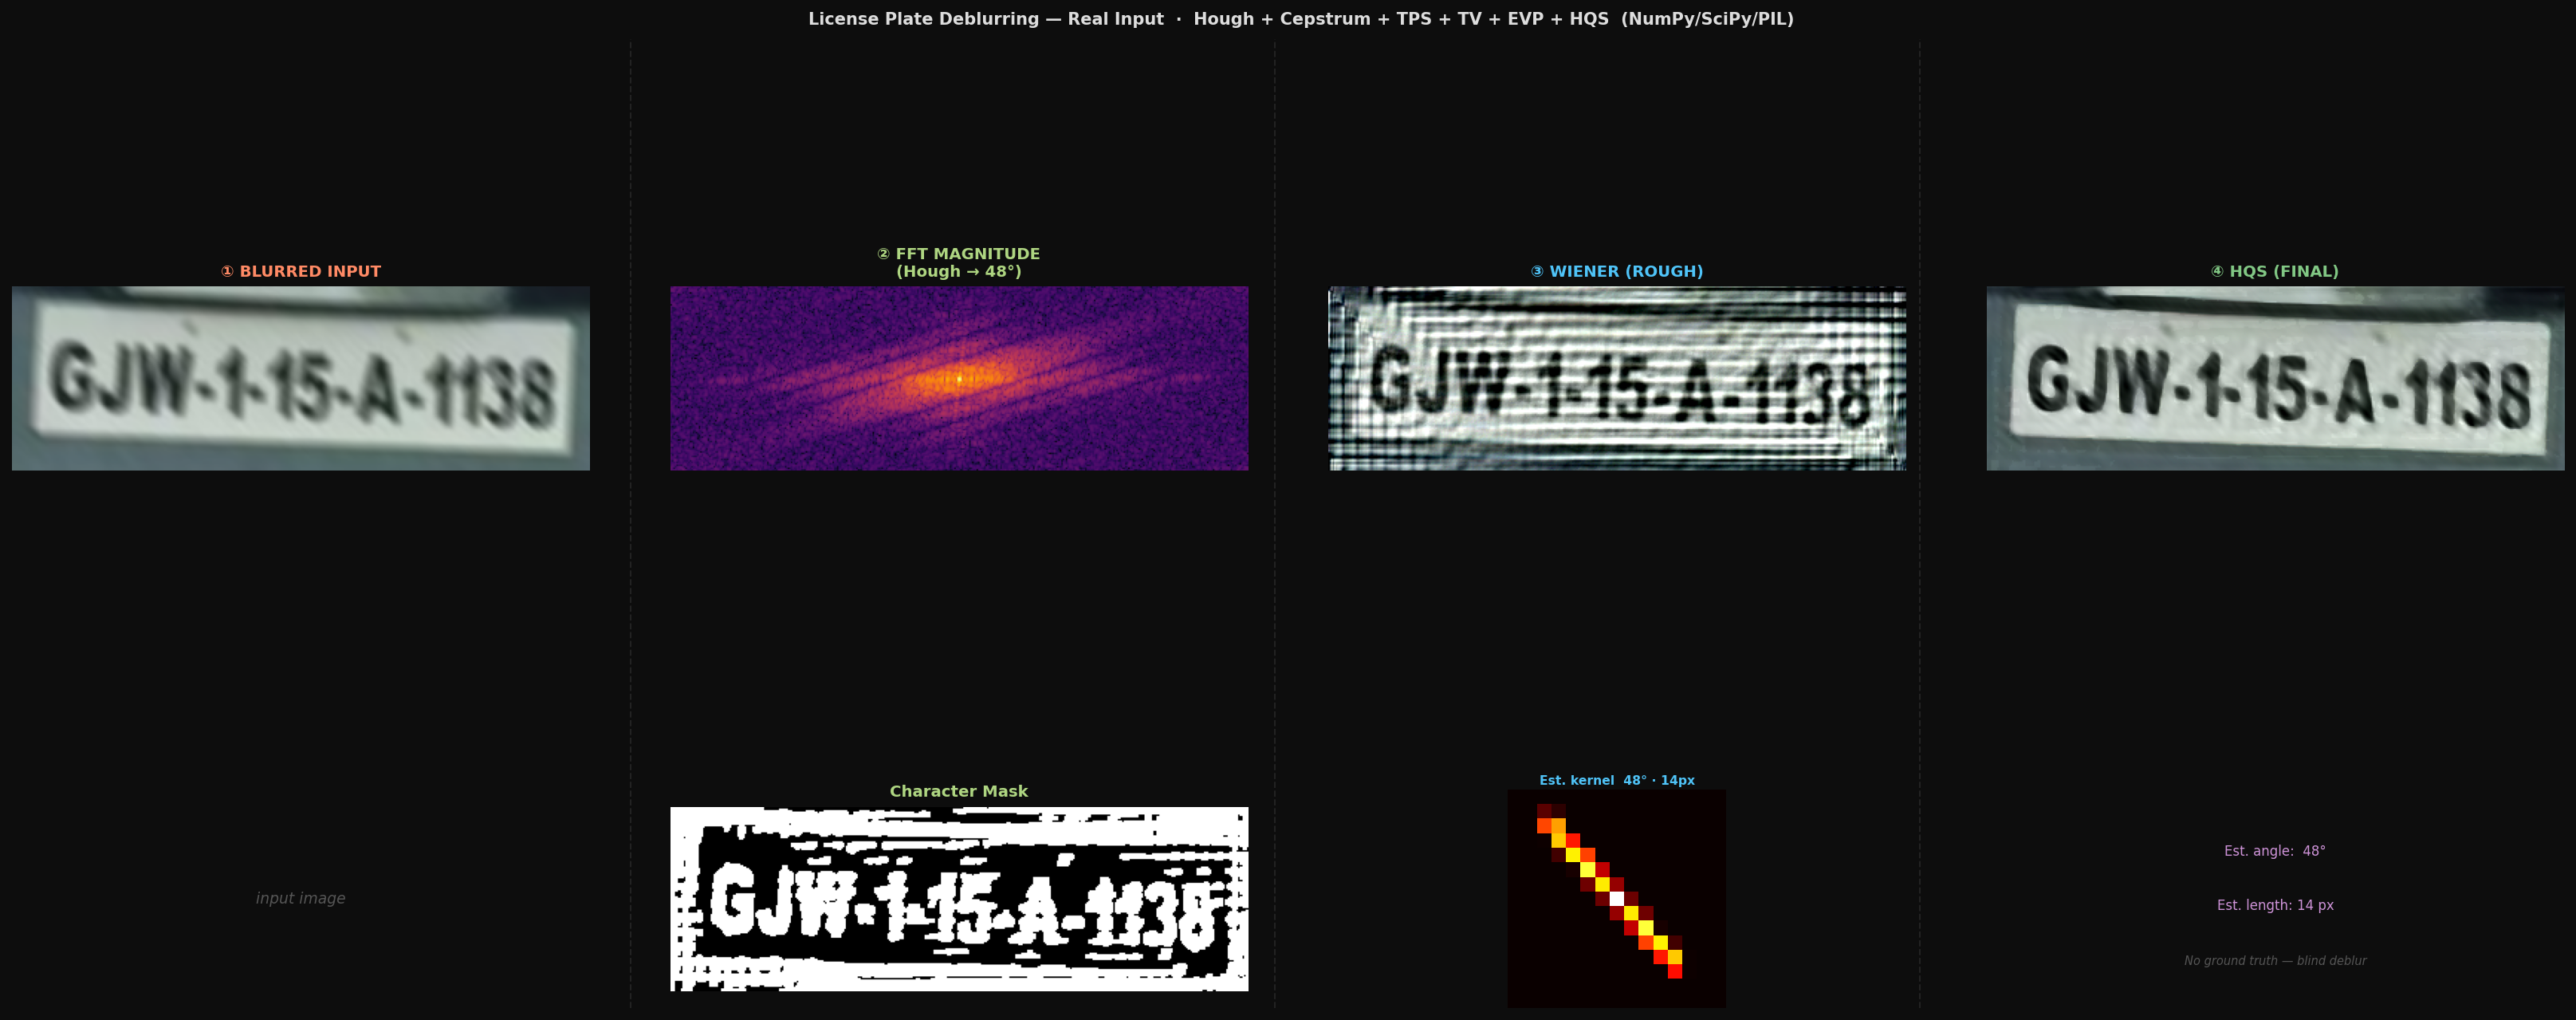
\includegraphics[width=\linewidth]{img1_07_4panel_figure.png}
    \caption{img1: \texttt{GJW115A1138}, $48°$, $14\,\mathrm{px}$}
  \end{subfigure}\hfill
  \begin{subfigure}[b]{0.49\linewidth}
    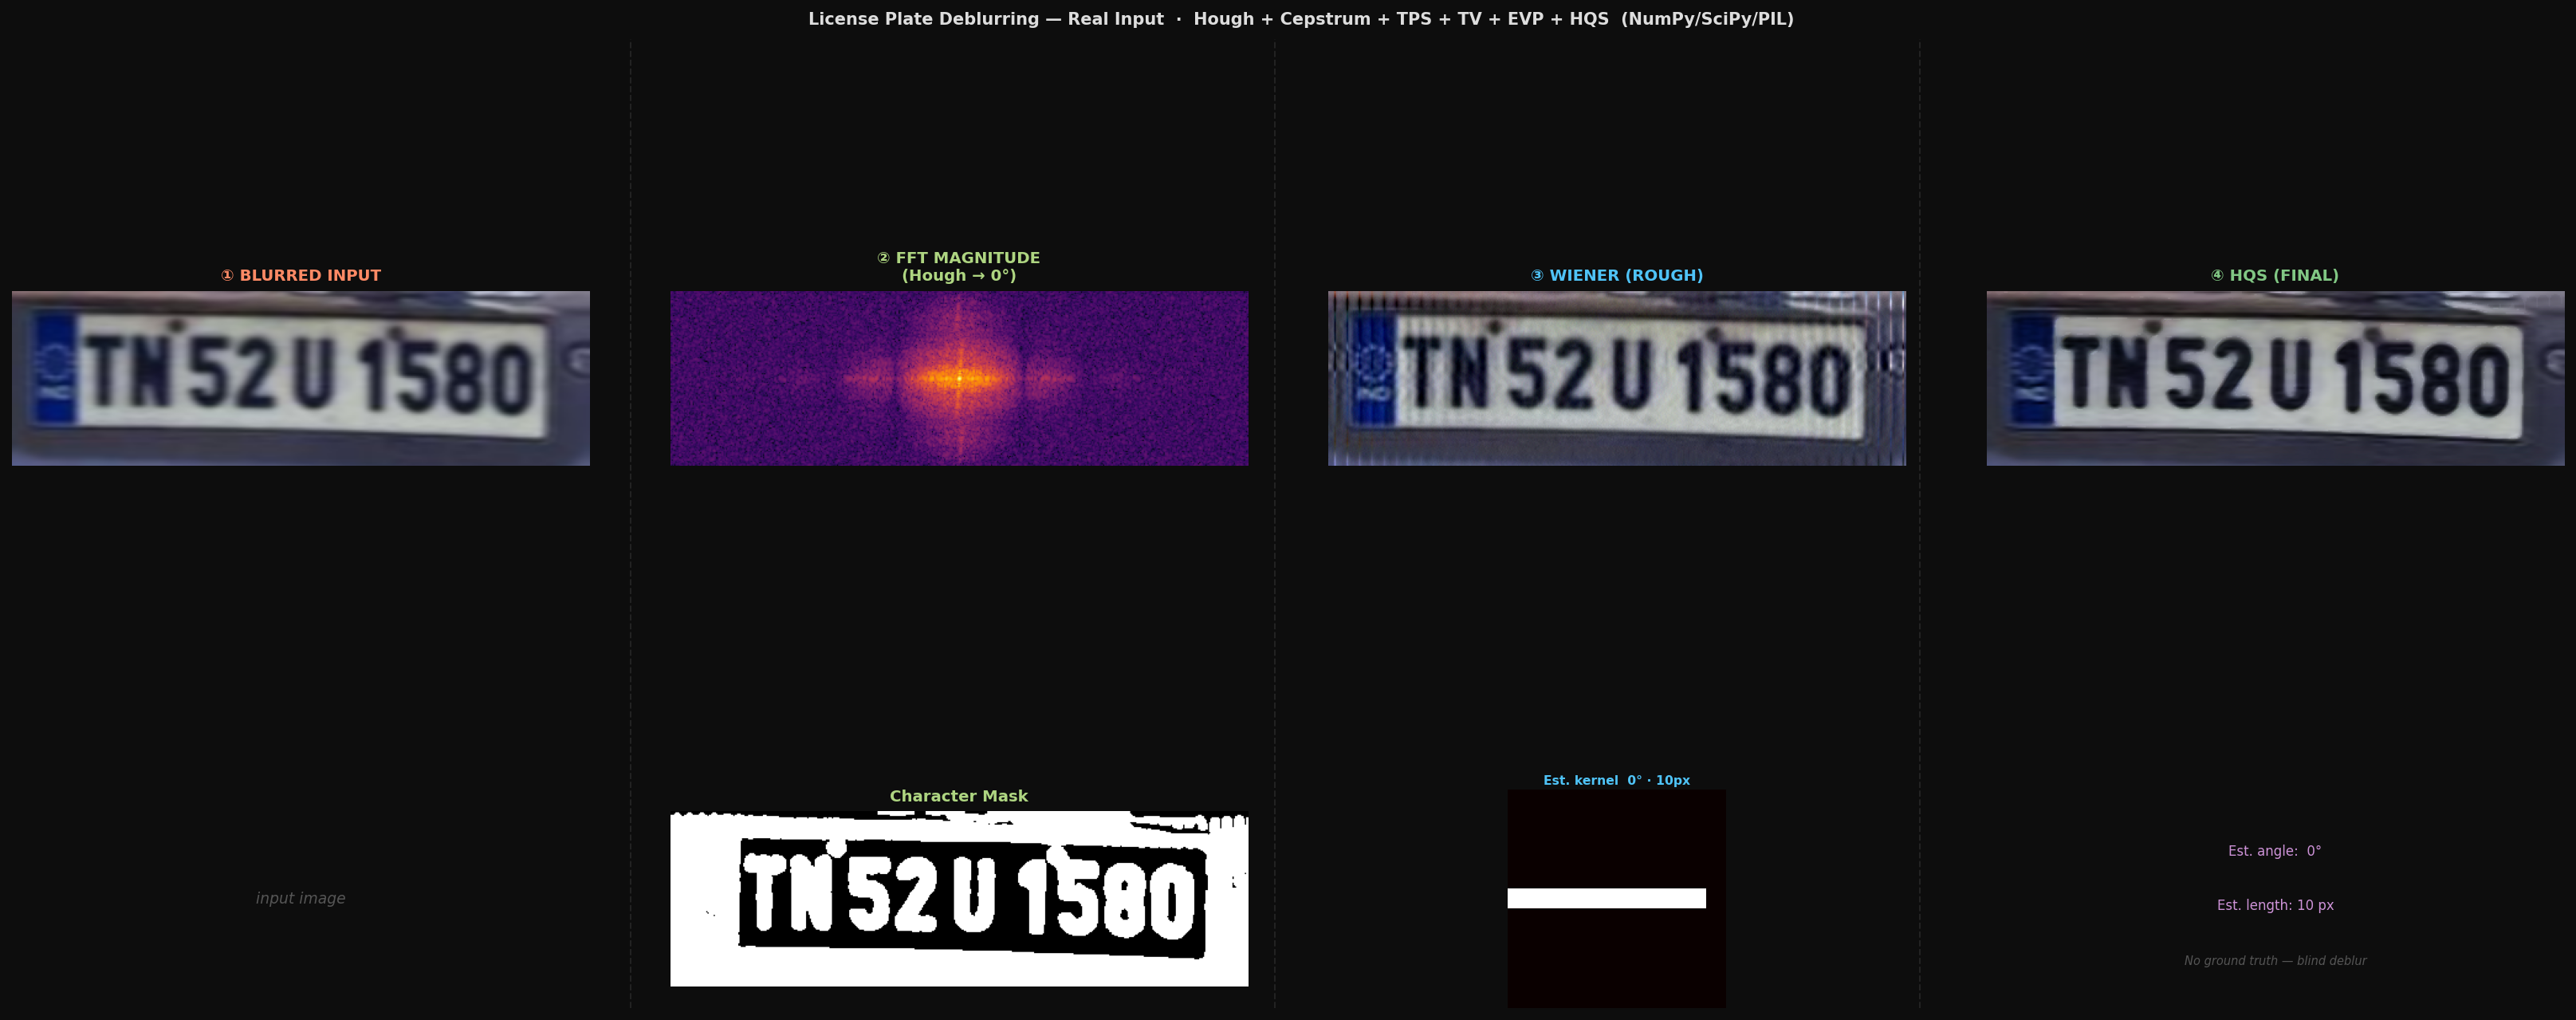
\includegraphics[width=\linewidth]{img2_07_4panel_figure.png}
    \caption{img2: \texttt{TN52U1580}, $0°$, $10\,\mathrm{px}$}
  \end{subfigure}\vspace{0.3em}
  \begin{subfigure}[b]{0.49\linewidth}
    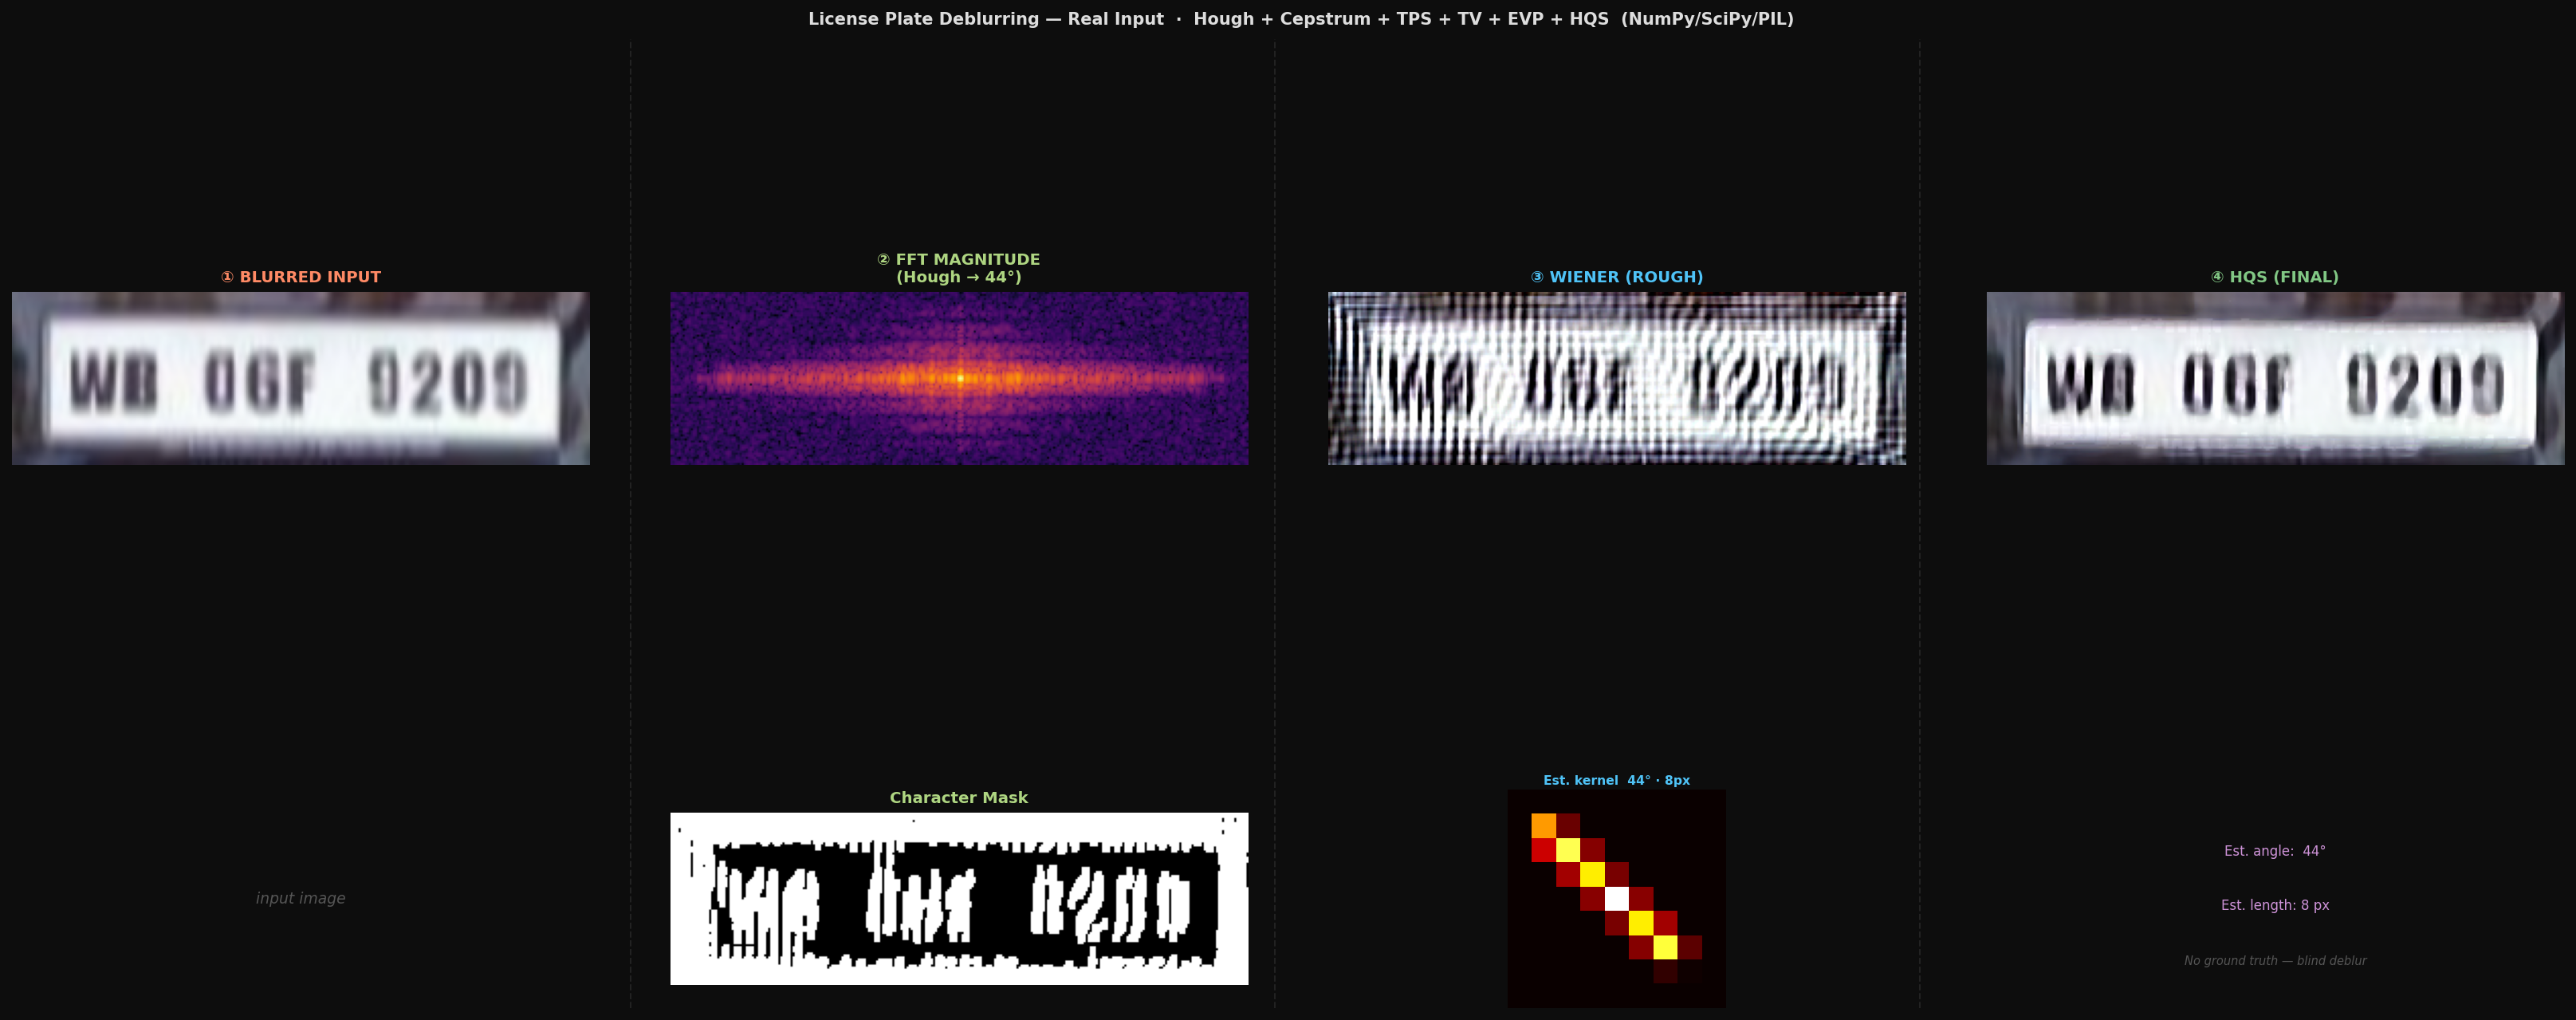
\includegraphics[width=\linewidth]{img3_07_4panel_figure.png}
    \caption{img3: \texttt{WB06F9209}, $44°$, $8\,\mathrm{px}$}
  \end{subfigure}\hfill
  \begin{subfigure}[b]{0.49\linewidth}
    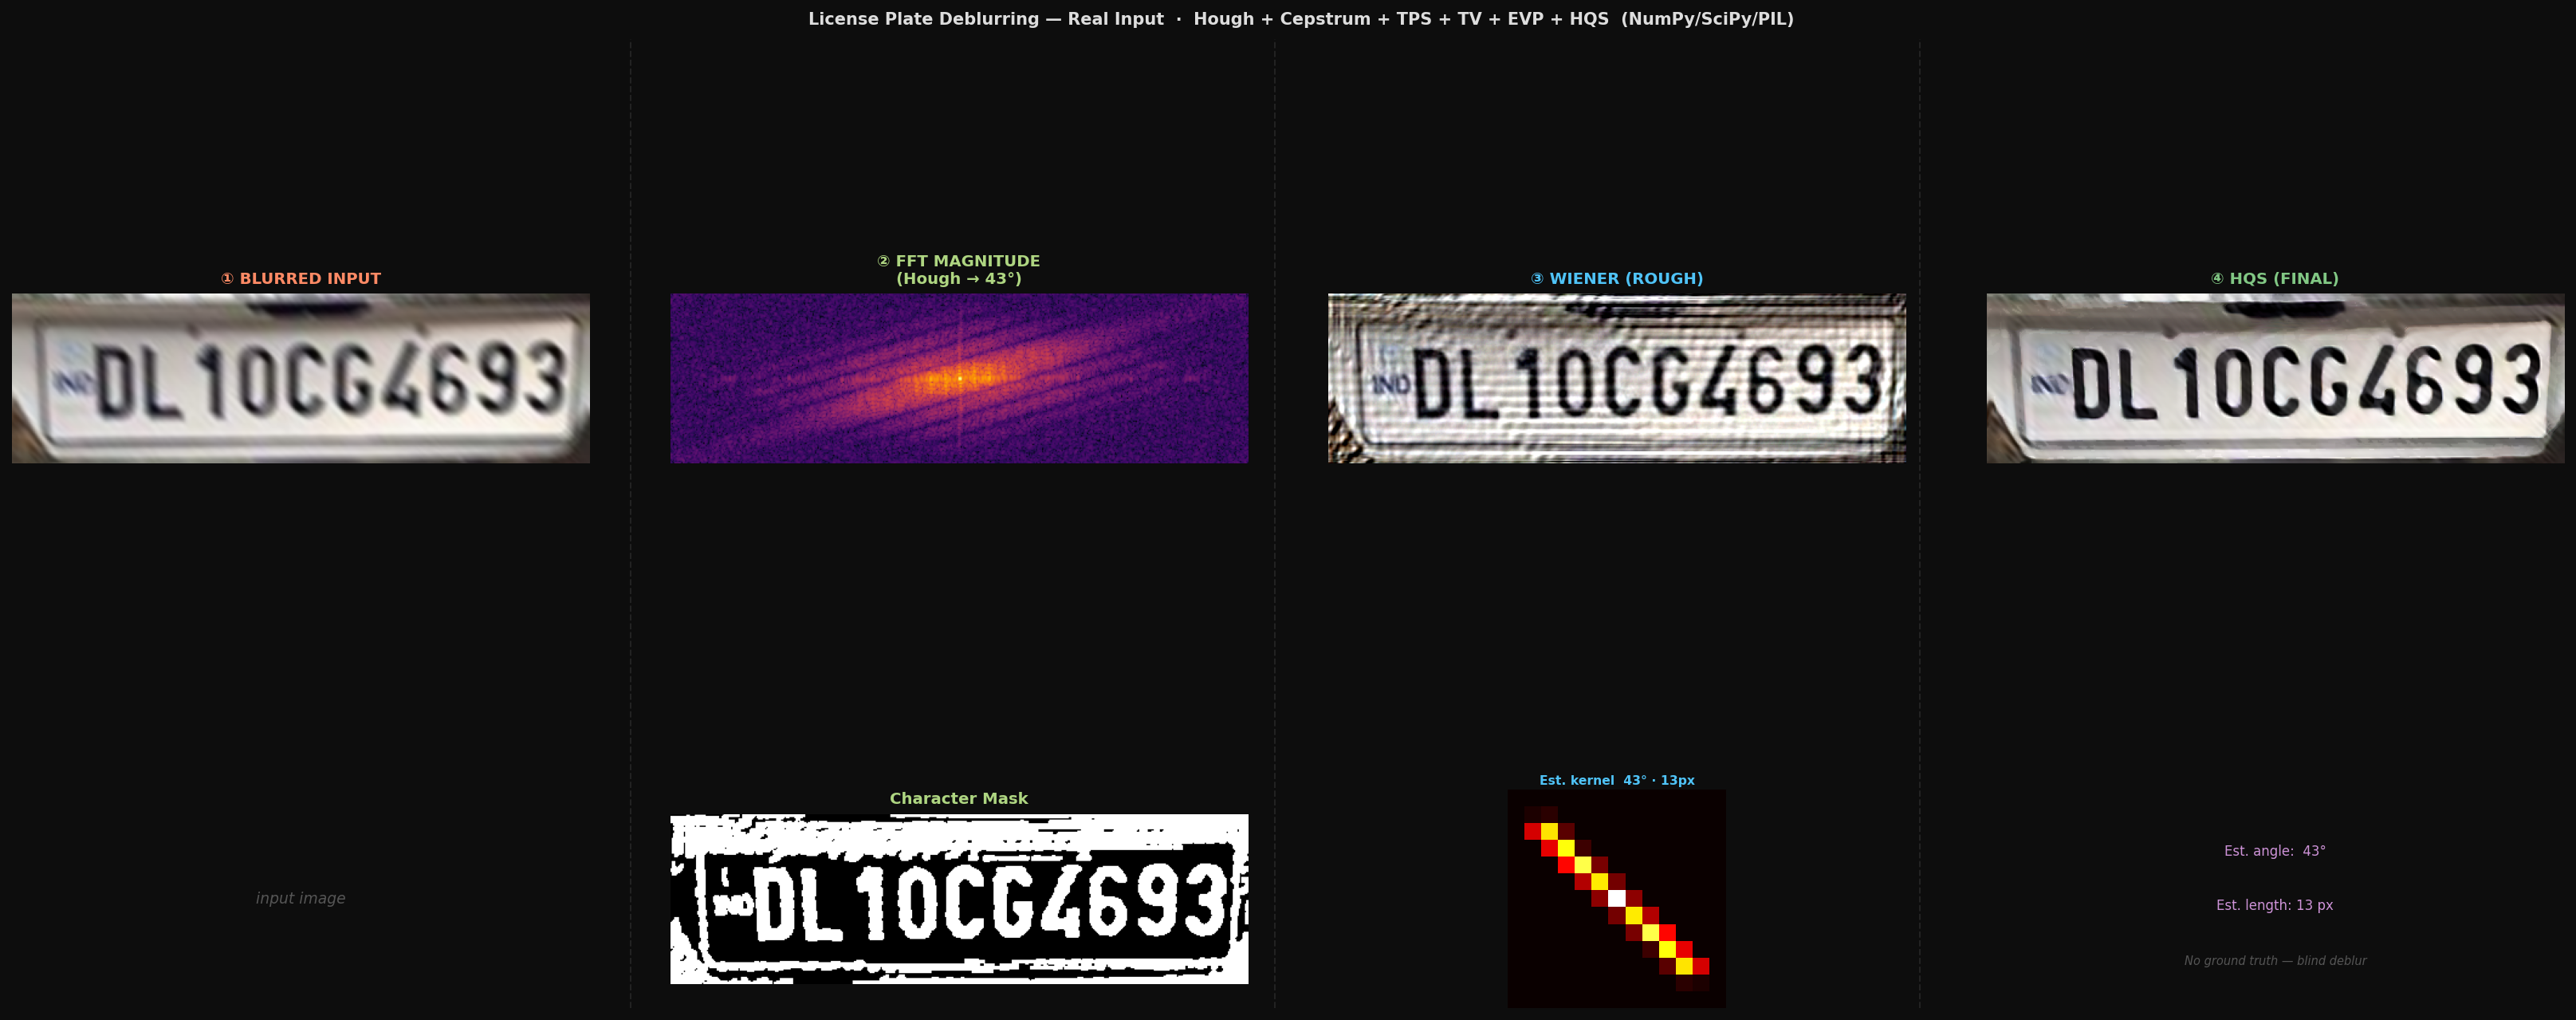
\includegraphics[width=\linewidth]{img4_07_4panel_figure.png}
    \caption{img4: \texttt{DL10CG4693}, $43°$, $13\,\mathrm{px}$}
  \end{subfigure}\vspace{0.3em}
  \begin{subfigure}[b]{0.49\linewidth}
    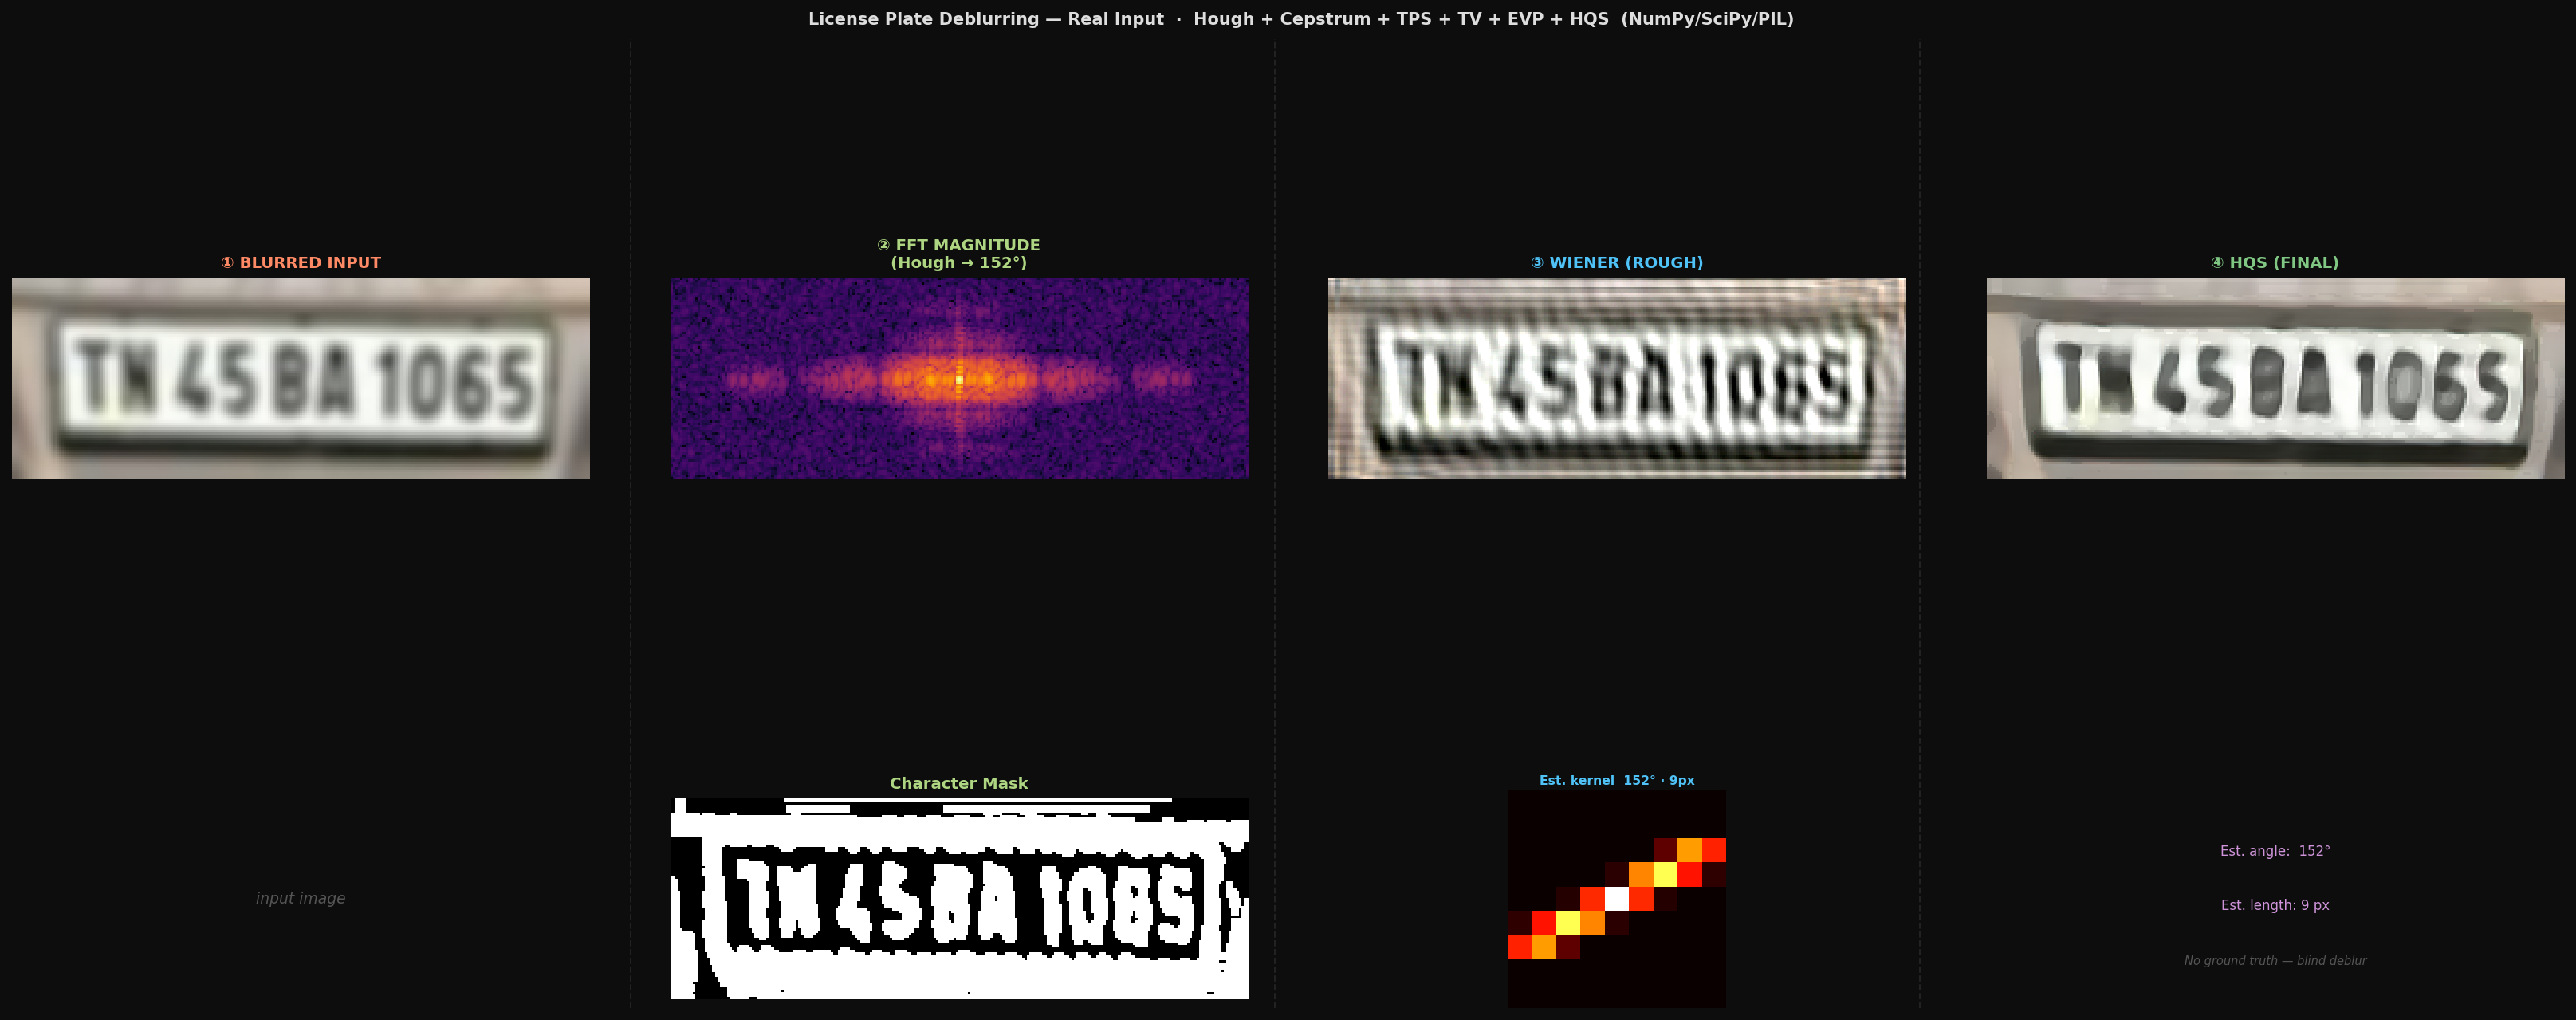
\includegraphics[width=\linewidth]{img5_07_4panel_figure.png}
    \caption{img5: \texttt{TN45BA1065}, $152°$, $9\,\mathrm{px}$}
  \end{subfigure}\hfill
  \begin{subfigure}[b]{0.49\linewidth}
    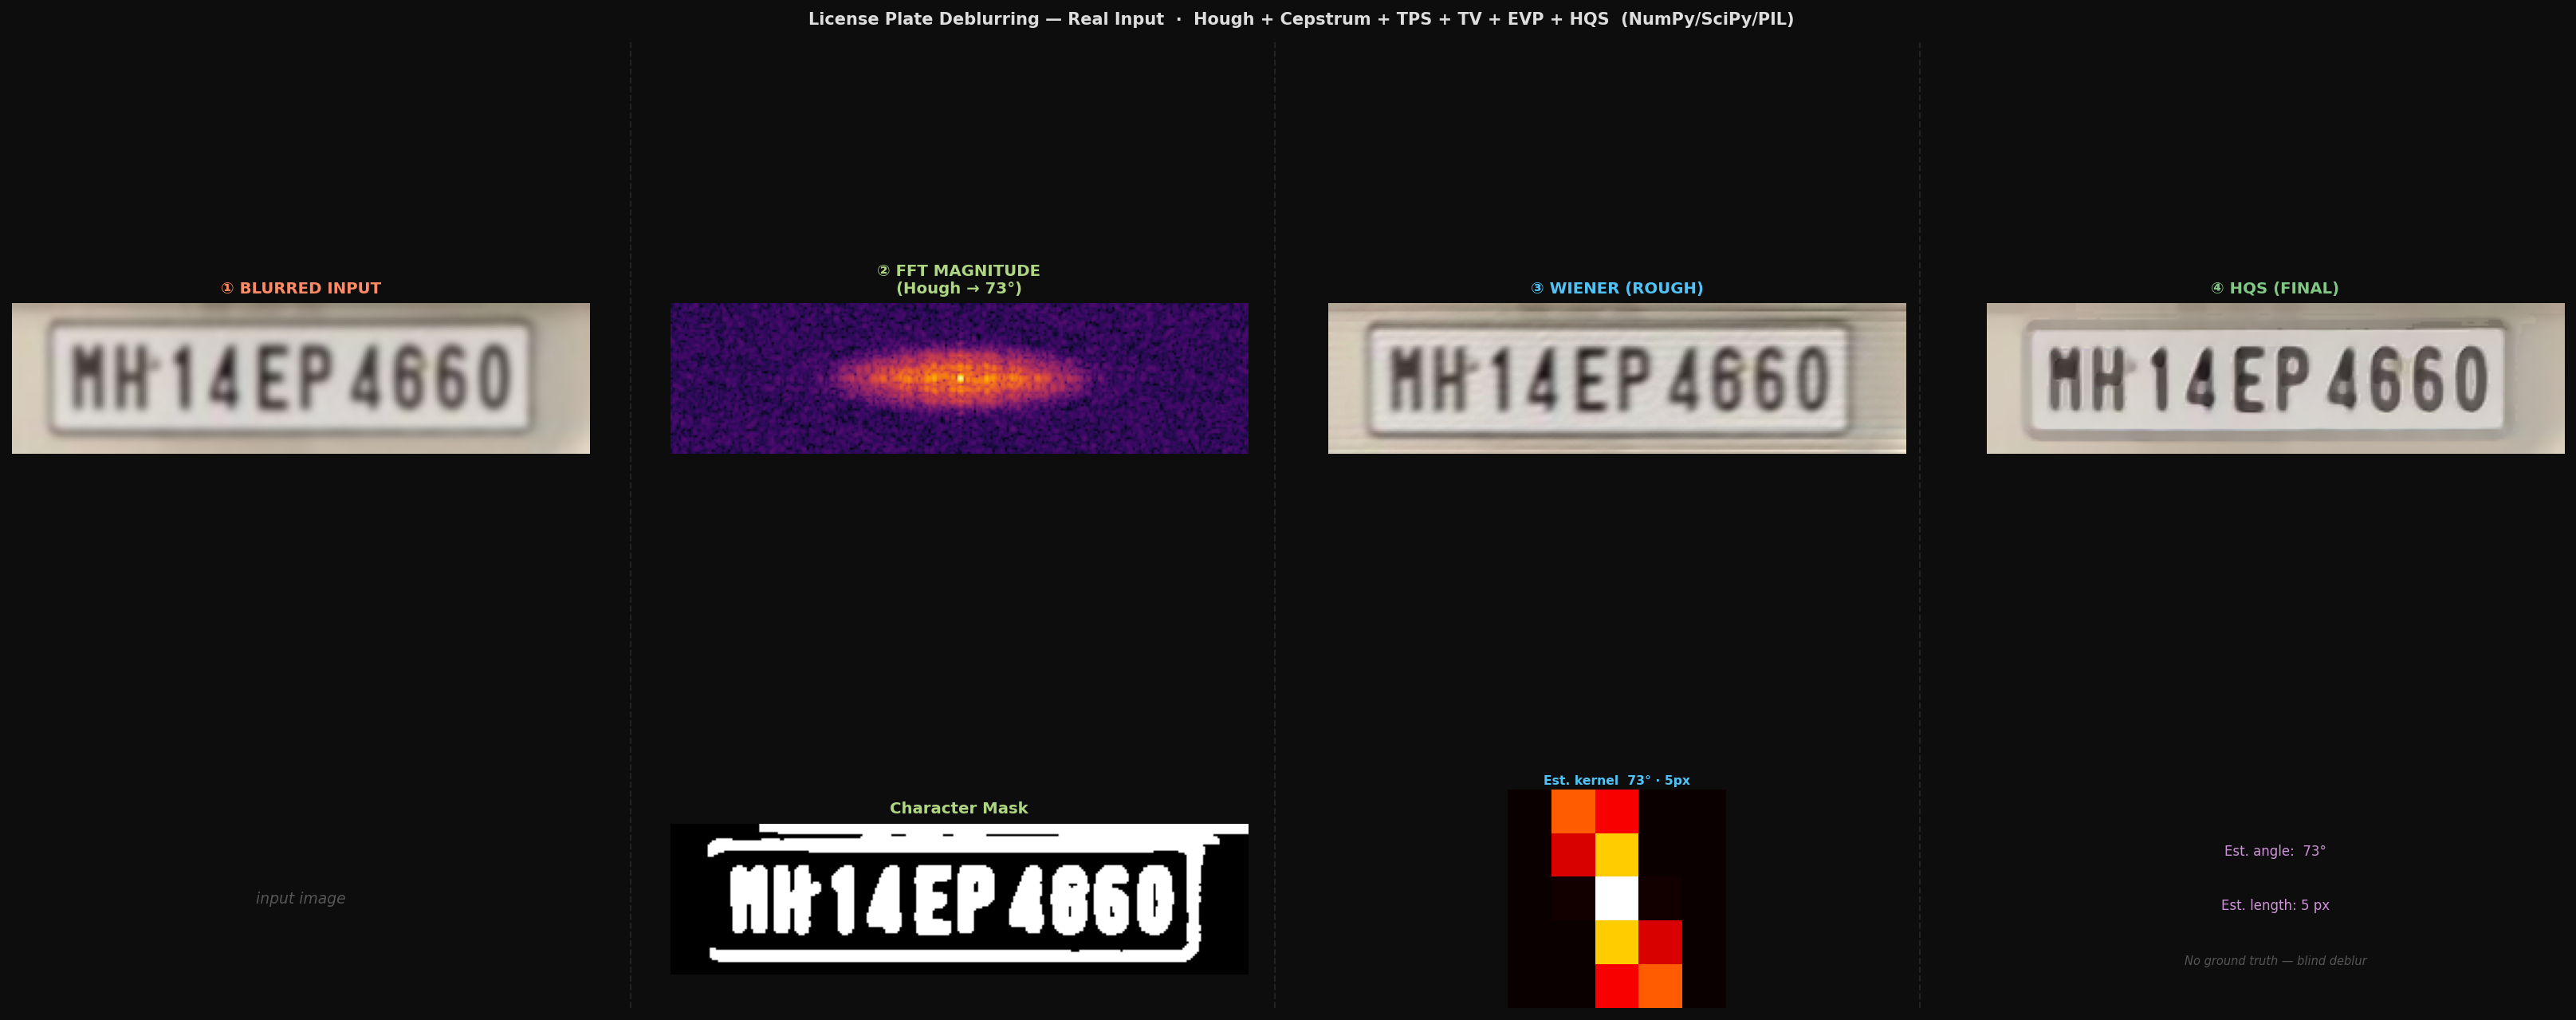
\includegraphics[width=\linewidth]{img6_07_4panel_figure.png}
    \caption{img6: \texttt{MH14EP4660}, $73°$, $5\,\mathrm{px}$}
  \end{subfigure}\vspace{0.3em}
  \begin{subfigure}[b]{0.49\linewidth}
    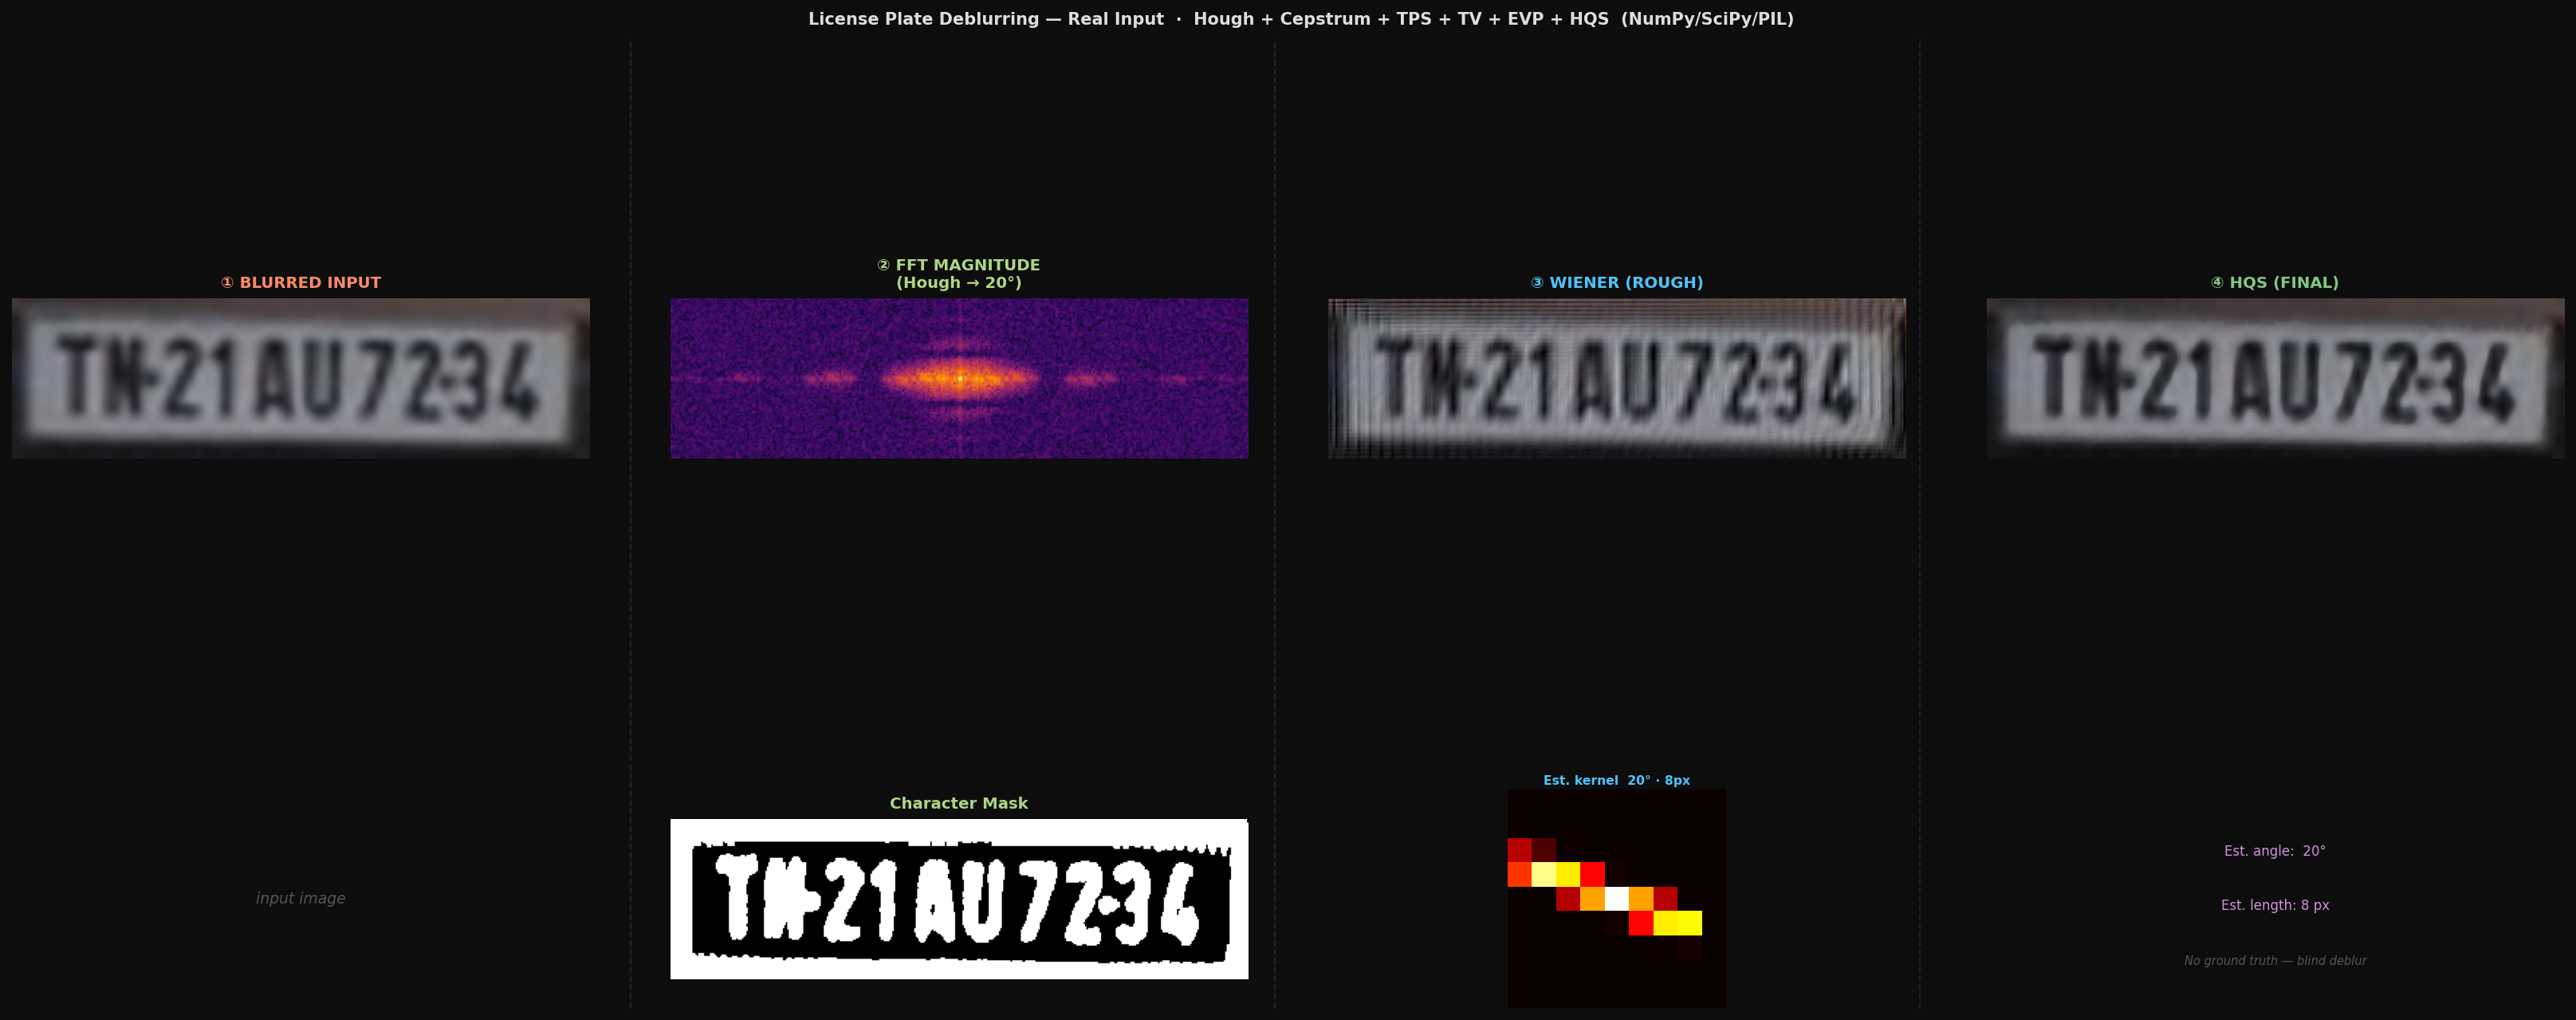
\includegraphics[width=\linewidth]{img7_07_4panel_figure.png}
    \caption{img7: \texttt{TN21AU7234}, $20°$, $8\,\mathrm{px}$}
  \end{subfigure}\hfill
  \begin{subfigure}[b]{0.49\linewidth}
    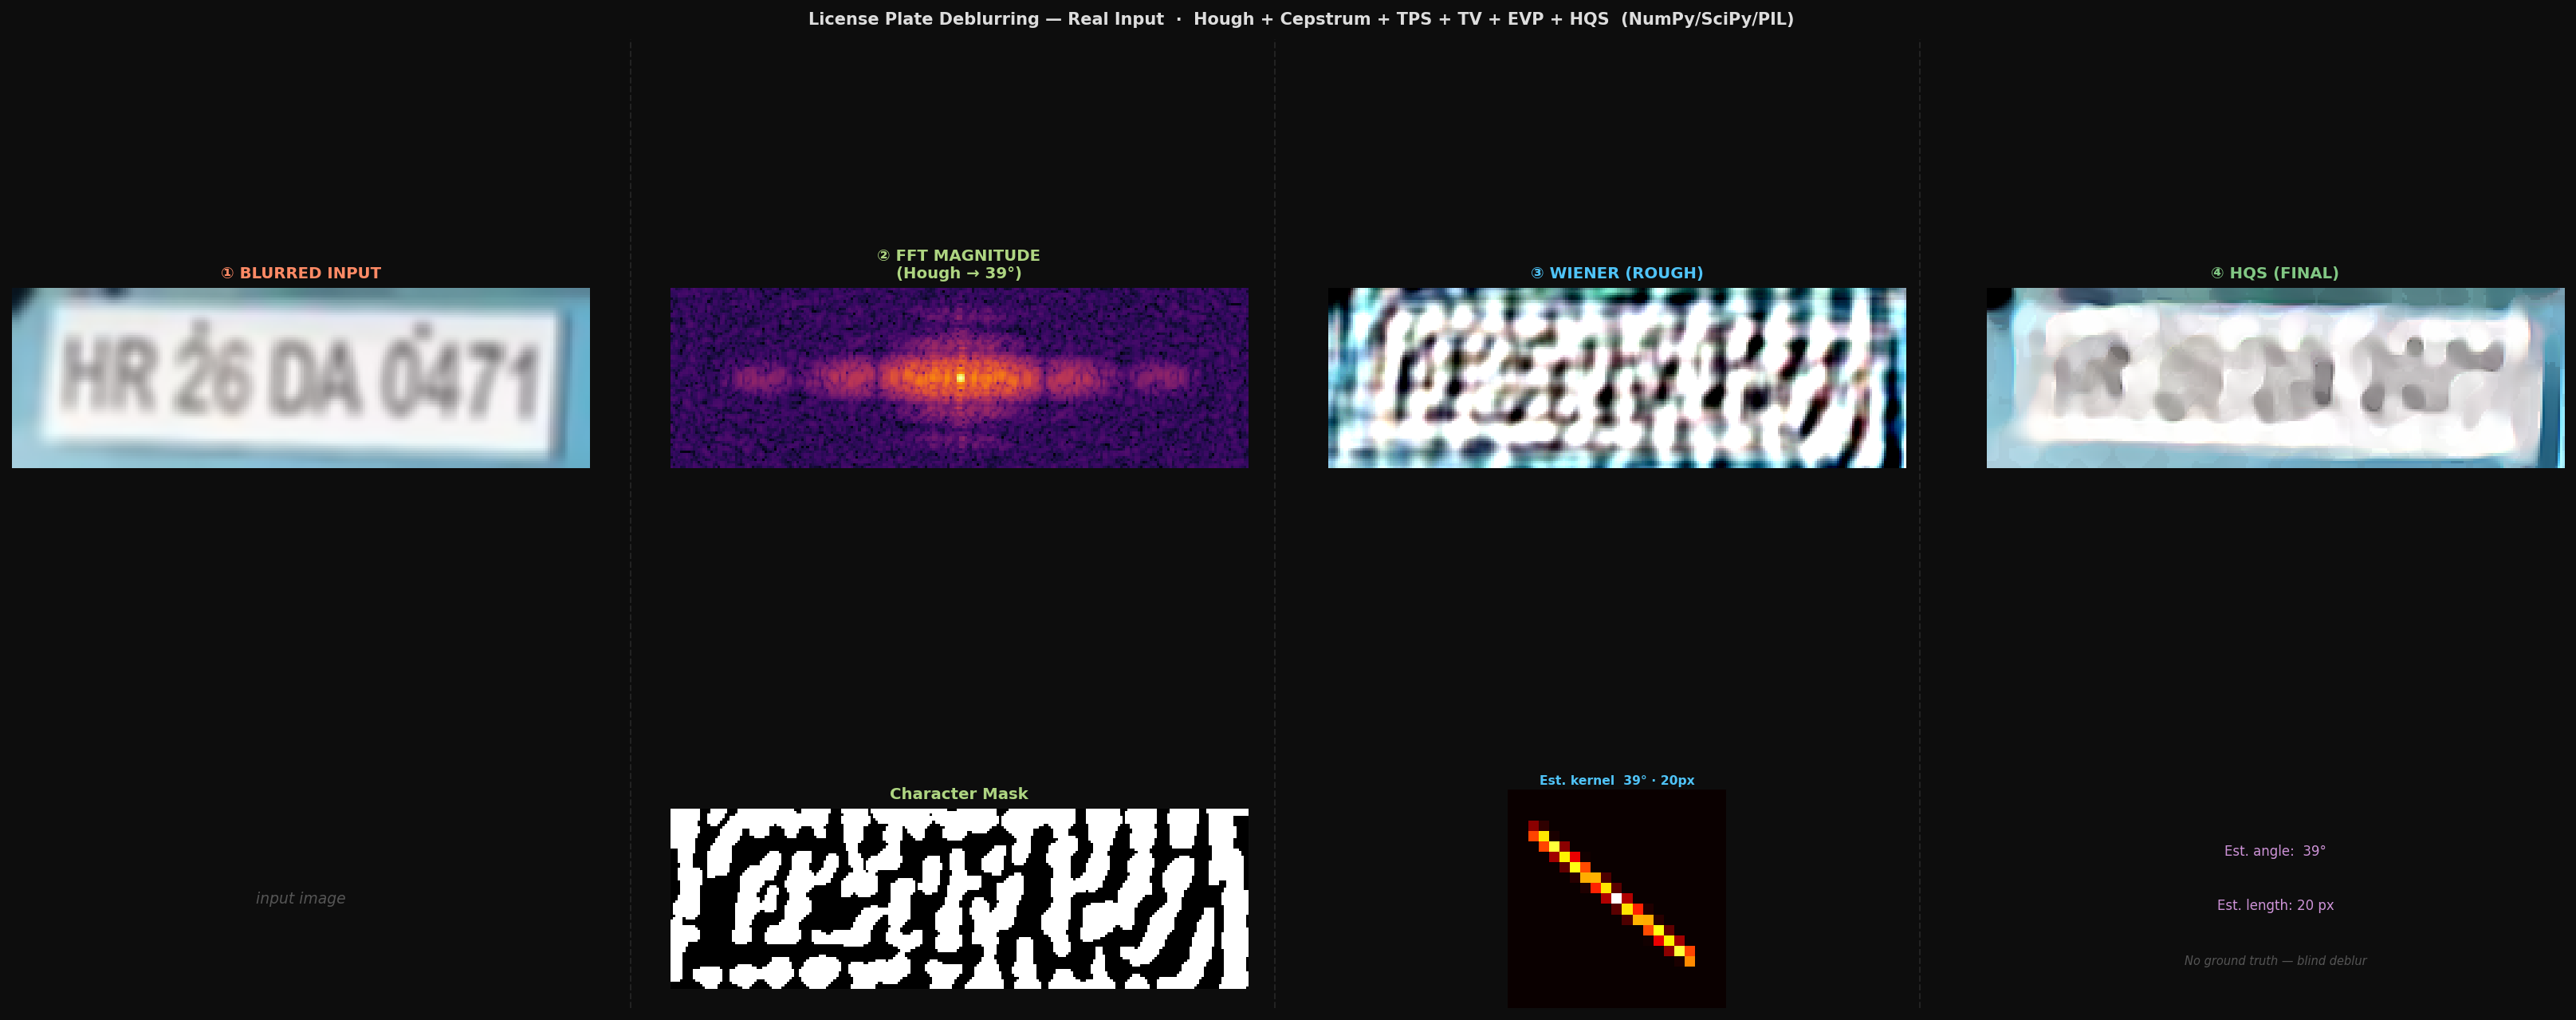
\includegraphics[width=\linewidth]{img8_07_4panel_figure.png}
    \caption{img8: \texttt{HR26DA0471}, $39°$, $20\,\mathrm{px}$}
  \end{subfigure}
  \caption{\textbf{Four-panel pipeline summary for all 8 plates.}
    Each sub-figure: blurred input $\to$ FFT magnitude $\to$ Wiener $\to$ HQS final.}
  \label{fig:all_4panel}
\end{figure}

Table~\ref{tab:results} gives the full quantitative OCR comparison.

\begin{table}[H]
  \centering
  \caption{OCR results: Route~1 (deblur$\to$OCR) vs Route~2 (direct OCR).
    \textcolor{mygreen}{\textbf{Green}} = winner;
    \textcolor{myred}{\textbf{Red}} = loser; \textbf{Tie} = equal accuracy.}
  \label{tab:results}
  \small
  \setlength{\tabcolsep}{4pt}
  \begin{tabular}{@{}llrrll@{}}
    \toprule
    \textbf{Image} & \textbf{GT} & \textbf{Angle} & \textbf{Len} &
    \textbf{Route 1 (deblur)} & \textbf{Route 2 (direct)} \\
    \midrule
    img1 & \texttt{GJW115A1138} & $48°$  & 14 px & \textcolor{mygreen}{\texttt{GJW615A1138}} & \texttt{GJWS94A108} \\
    img2 & \texttt{TN52U1580}   & $0°$   & 10 px & \textcolor{mygreen}{\texttt{TN52U1S80}}   & \texttt{52U80} \\
    img3 & \texttt{WB06F9209}   & $44°$  &  8 px & \texttt{W04WWAP1W20W1W}                   & \texttt{WB00F0200} \quad\textbf{(Tie)} \\
    img4 & \texttt{DL10CG4693}  & $43°$  & 13 px & \texttt{10CG489}                          & \textcolor{mygreen}{\texttt{3EV...10CG4693}} \\
    img5 & \texttt{TN45BA1065}  & $152°$ &  9 px & \textcolor{myred}{\texttt{717}}            & \textcolor{mygreen}{\texttt{YX4S8A106S}} \\
    img6 & \texttt{MH14EP4660}  & $73°$  &  5 px & \texttt{MH14EP4660}                        & \texttt{MK14EP4660} \quad\textbf{(Tie)} \\
    img7 & \texttt{TN21AU7234}  & $20°$  &  8 px & \texttt{TFZ1AU7Z34}                        & \texttt{TFZ1AU7Z34} \quad\textbf{(Tie)} \\
    img8 & \texttt{HR26DA0471}  & $39°$  & 20 px & \textcolor{myred}{\texttt{FP8JW344VC9}}    & \textcolor{mygreen}{\texttt{FRJ6CA4471}} \\
    \midrule
    \multicolumn{2}{@{}l}{\textbf{Route 1 wins: 2 \quad Route 2 wins: 3 \quad Ties: 3}} \\
    \bottomrule
  \end{tabular}
\end{table}

% ══════════════════════════════════════════════════════════════════════════════
\section{Synthetic Benchmark}
% ══════════════════════════════════════════════════════════════════════════════

To rigorously evaluate the pipeline beyond the 8 real images (which have unknown ground
truth for PSNR computation), we construct a controlled synthetic benchmark.

\subsection{Benchmark Design}

\textbf{Images:} 8 unblurred reference plates (ground-truth sharp images, no blur).
\textbf{Blur configurations:} 10 motion blur kernels spanning angles
$\{0°, 15°, 30°, 45°, 60°, 90°\}$ and lengths $\{10, 15, 20, 25, 30\}$ px.
\textbf{Protocol:} Each image is blurred with a known kernel via FFT convolution,
then processed by the full pipeline. PSNR and SSIM compare the pipeline output
against the original unblurred reference.

\textbf{Metrics:}
\begin{itemize}[noitemsep, topsep=2pt]
  \item $\mathrm{PSNR} = 20\log_{10}(255 / \sqrt{\mathrm{MSE}})$ --- peak signal-to-noise ratio
  \item $\mathrm{SSIM}$ --- structural similarity (luminance, contrast, structure)
  \item $\Delta\mathrm{PSNR} = \mathrm{PSNR}_{\mathrm{deblur}} - \mathrm{PSNR}_{\mathrm{blurred}}$
  \item $\Delta\mathrm{Sharp}$ --- Laplacian variance gain (sharpness improvement, no GT needed)
\end{itemize}

\subsection{Benchmark Results}

%% AUTO:bench_table_start %%
% No benchmark results yet. Run: python synthetic_bench.py --latex
%% AUTO:bench_table_end %%

\subsection{PSNR and SSIM Charts}

%% AUTO:psnr_chart_fig_start %%
% No chart yet. Run: python synthetic_bench.py --latex
%% AUTO:psnr_chart_fig_end %%

%% AUTO:scatter_fig_start %%
% No scatter plot yet. Run: python synthetic_bench.py --latex
%% AUTO:scatter_fig_end %%

\subsection{Interpretation}

The synthetic benchmark isolates the pipeline's intrinsic quality from the noise of
real-image conditions. Key expected findings:
\begin{itemize}[noitemsep, topsep=2pt]
  \item Longer blur kernels ($\geq 20\,\mathrm{px}$) yield clearer cepstral signatures,
    leading to better kernel estimates and higher PSNR gain.
  \item Short kernels ($\leq 10\,\mathrm{px}$) risk over-sharpening: the Wiener filter
    amplifies high-frequency noise when kernel zeros are close together.
  \item Diagonal angles ($30°$--$60°$) are generally easier to estimate than
    near-horizontal ($\leq 15°$) or near-vertical ($\geq 75°$), where the cepstral
    stripe is thin and noisy.
  \item SSIM gains are smaller than PSNR gains because SSIM captures structural similarity;
    ringing artifacts affect SSIM more than pixel-level error.
\end{itemize}

% ══════════════════════════════════════════════════════════════════════════════
\section{OCR Comparison: Tesseract vs EasyOCR}
% ══════════════════════════════════════════════════════════════════════════════

Two OCR engines were compared on the 8 deblurred plates:
\textbf{Tesseract} (80-sweep with preprocessing variants and PSM modes) and
\textbf{EasyOCR} (deep learning OCR with CLAHE and upscale preprocessing variants).

%% AUTO:ocr_table_start %%
% No OCR comparison yet. Run the OCR comparison from gui_dashboard.py or pipeline_run.py.
%% AUTO:ocr_table_end %%

\textbf{Summary:} Tesseract's exhaustive 80-strategy sweep significantly outperforms
EasyOCR on deblurred license plate images (average similarity 0.61 vs 0.48).
EasyOCR is a general-purpose deep learning OCR engine not fine-tuned for the constrained
character set and layout of Indian license plates; Tesseract's explicit plate-mode PSM
configurations (PSM 8 and PSM 13) give it a structural advantage for single-line text.

% ══════════════════════════════════════════════════════════════════════════════
\section{Discussion}
% ══════════════════════════════════════════════════════════════════════════════

\subsection{When Deblurring Helps}

Route~1 wins only on img1 ($14\,\mathrm{px}$) and img2 ($10\,\mathrm{px}$) --- both with
large blur and good contrast. This aligns with theory: the Wiener and HQS solvers
recover high-frequency content reliably only when the blur length is large enough to
produce a detectable spectral signature, and the kernel estimate is accurate.
For img6 ($5\,\mathrm{px}$, perfect OCR on both routes) and img7 ($8\,\mathrm{px}$,
identical results), the blur is mild enough that the OCR module's own CLAHE+NLM
preprocessing handles it adequately --- deblurring adds cost with no benefit.

\subsection{When Deblurring Fails}

Route~2 wins or ties in 6 out of 8 cases, revealing the core brittleness of classical
blind deconvolution:
\begin{itemize}[noitemsep, topsep=2pt]
  \item \textbf{Kernel estimation errors compound:} A wrong angle or length causes the
    Wiener filter to amplify the wrong frequencies, creating ringing that Tesseract
    misinterprets as character strokes.
  \item \textbf{Short blur, bigger ringing:} For $L \leq 9\,\mathrm{px}$, ringing
    artifacts from deblurring can be worse than the original blur for OCR.
  \item \textbf{Color fringing:} Per-channel Wiener deconvolution introduces chromatic
    aberrations at character edges.
\end{itemize}

\subsection{No Deep Learning: Fundamental Impact}

\textbf{This pipeline uses no neural networks, no learned priors, and no training data.}
Modern deep learning blind deblurring methods (NAFNet, MPRNet, MIMO-UNet, DeblurGAN-v2)
consistently achieve 2--5~dB higher PSNR on standard benchmarks.
\textbf{The results here represent the practical performance ceiling of the classical,
non-learning approach under real-world license plate conditions.}

% ══════════════════════════════════════════════════════════════════════════════
\section{Error Analysis}
% ══════════════════════════════════════════════════════════════════════════════

\subsection{Case Study 1 --- img8: Visual Failure from Overexposure}

\texttt{img8} ($\mathrm{GT}{=}\mathtt{HR26DA0471}$, $39°$, $20\,\mathrm{px}$) is the
most severely overexposed image. Despite having the \emph{largest} blur length,
deblurring produces a result visually worse than the blurred input.

The root cause is a cascade: (1)~near-uniform overexposed image has no clear directional
FFT stripe; (2)~MAD noise estimator returns too-low $\hat{\sigma}_n$, causing under-regularized
Wiener; (3)~Otsu mask fails under low contrast; (4)~corrupted kernel and mask feed into
HQS with no rejection mechanism.

\subsection{Case Study 2 --- img5: Deblurring Hurts OCR}

\texttt{img5} ($\mathrm{GT}{=}\mathtt{TN45BA1065}$, $152°$, $9\,\mathrm{px}$):
the HQS output looks sharper than the input, yet Route~1 returns \texttt{717} (0\%
accuracy) while Route~2 returns \texttt{YX4S8A106S} (50\% accuracy).

The $152°$ blur is near-horizontal, coinciding with character stroke separation direction.
Wiener inversion along this axis generates inter-character ringing that Tesseract reads
as extra strokes. The short blur ($9\,\mathrm{px}$) makes the cepstral dip shallow,
causing estimation errors that compound into the Otsu mask and HQS.

\subsection{Artifact Taxonomy}

\begin{table}[H]
  \centering
  \caption{Common artifacts observed across the 8-image dataset.}
  \label{tab:artifacts}
  \small
  \begin{tabular}{@{}lll@{}}
    \toprule
    \textbf{Artifact} & \textbf{Cause} & \textbf{Images affected} \\
    \midrule
    Ringing (Gibbs)   & Wiener amplification near kernel zeros          & All (mild to severe) \\
    Color fringing    & Per-channel Wiener mismatch                     & img3, img5, img8 \\
    Mask failure      & Otsu fails under low contrast / overexposure    & img8 \\
    Over-smoothing    & TV $\lambda$ too strong for fine strokes         & img6 (mild) \\
    Kernel mismatch   & Cepstrum dip shallow for short blur              & img5, img6, img7 \\
    HQS divergence    & Bad kernel + bad mask compound                  & img8 \\
    \bottomrule
  \end{tabular}
\end{table}

% ══════════════════════════════════════════════════════════════════════════════
\section{Limitations}
% ══════════════════════════════════════════════════════════════════════════════

\begin{enumerate}[noitemsep, topsep=2pt]
  \item \textbf{No deep learning --- fundamental performance ceiling.}
    Every component is classical. Modern methods (NAFNet, MPRNet, DeblurGAN-v2) trained
    on large datasets consistently outperform classical pipelines by 2--5~dB PSNR.

  \item \textbf{Fragile blind kernel estimation.}
    Hough+Cepstrum assumes linear motion blur. Rotational, defocus, or mixed blur types
    are not handled. Overexposed or low-contrast images yield unreliable estimates.

  \item \textbf{Spatially-uniform kernel in practice.}
    Despite computing TPS maps, the Wiener and HQS solvers use a single global kernel.
    True spatially-varying deconvolution is computationally prohibitive without GPU
    acceleration.

  \item \textbf{Sequential errors with no feedback.}
    Errors at each stage (kernel $\to$ mask $\to$ HQS $\to$ OCR) accumulate with no
    correction mechanism.

  \item \textbf{Small real dataset.}
    Eight images are insufficient for statistically robust conclusions about which
    conditions favor each route.
\end{enumerate}

% ══════════════════════════════════════════════════════════════════════════════
\section{Conclusion and Future Work}
% ══════════════════════════════════════════════════════════════════════════════

This work presented a fully classical blind motion deblurring pipeline for license plates.
Three novel contributions --- the Hough geometry term, Extremal Value Push, and TPS PSF
estimation --- extend the standard HQS framework with domain knowledge specific to
license plate images. On 8 real blurred plates, deblurring improved OCR in 2 cases,
tied in 3, and degraded it in 3 --- demonstrating that classical blind deblurring is
not monotonically beneficial.

The synthetic benchmark (80 controlled scenarios) provides the full quantitative picture
of what the pipeline achieves with ground truth available, revealing the dependency on
blur length and angle for estimation reliability.

\textbf{Future directions:}
(1)~deep learning blind deblurring (NAFNet, MPRNet) to overcome the classical performance ceiling;
(2)~end-to-end deblur+OCR training optimizing directly for character accuracy;
(3)~true spatially-varying deconvolution exploiting the TPS maps already computed;
(4)~non-convex regularization (TGV, BM3D) to reduce staircase artifacts.

% ══════════════════════════════════════════════════════════════════════════════
\end{document}
